\chapter{Przegląd algorytmów wyszukujących cechy obrazów}
Poszukując algorytmów służących do lokalizowania cech charakterystycznych obrazów posłużono się badaniami \cite{IK111}, \cite{IK112}. Autor w oparciu o prace \cite{LIFDAS} dokonał zestawienia popularnych metod zaimplementowanych w służących do przetwarzania obrazów bibliotece OpenCV (wersje 2.2.0 i 2.3.1). Algorytmy były badane na testowym zbiorze obrazów przedstawionym na rysunku \ref{fig:zestaw_obrazow_start} poddanego przekształceniom programowym. Wyniki badań prezentują rezultaty od \ref{fig:Number-of-detected-features_thumb}, do \ref{fig:Percent-of-tracked-feature_thumb}.

\begin{figure}[!htb]
\begin{center}

\subfigure[Barbara]{
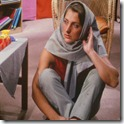
\includegraphics{pict/01/barbara_thumb.jpg}
\label{pict:01_Barbara}
}
\subfigure[Lena]{
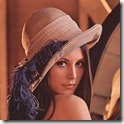
\includegraphics{pict/01/lena_thumb.jpg}
\label{pict:01_Lena}
}
\subfigure[Pepppers]{
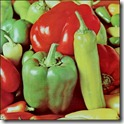
\includegraphics{pict/01/peppers_thumb.jpg}
\label{pict:01_Pepppers}
}
\subfigure[Mandril]{
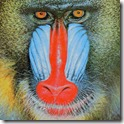
\includegraphics{pict/01/mandril_thumb.jpg}
\label{pict:01_Mandril}
}
\caption{Zestaw obrazów testowych do porównania algorytmów}
\label{fig:zestaw_obrazow_start}
\end{center}
\end{figure}

\begin{figure}[!htb]
\centering
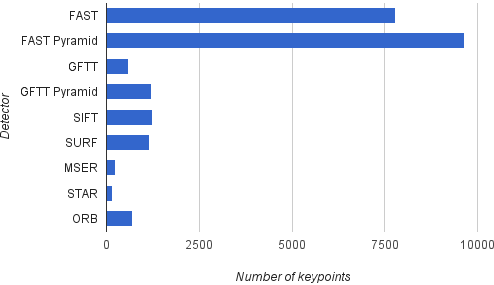
\includegraphics[height=66mm]{pict/01/Number-of-detected-features_thumb.png}
\caption{Liczba wykrytych cech}
\label{fig:Number-of-detected-features_thumb}
\end{figure}

\begin{figure}[!htb]
\centering
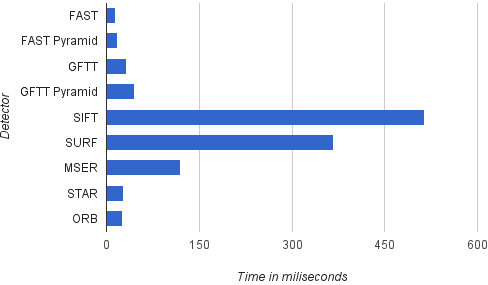
\includegraphics[height=66mm]{pict/01/Detection-cost_thumb.png}
\caption{czas potrzebny na wykrycie cechy}
\label{fig:Detection-cost_thumb}
\end{figure}
\begin{figure}[!htb]
\centering
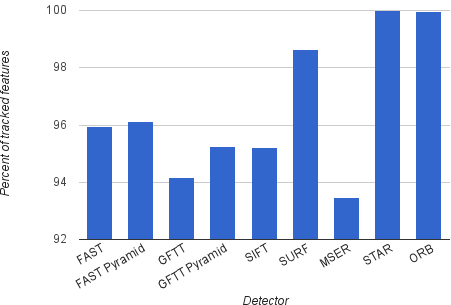
\includegraphics[height=66mm]{pict/01/Percent-of-tracked-feature_thumb.png}
\caption{Skuteczność śledzenia wyszukanych cech}
\label{fig:Percent-of-tracked-feature_thumb}
\end{figure}

\newpage


Na podstawie zaprezentowanych wyników wszystkie algorytmy możemy zaklasyfikować jako dobre, gdyż pozwalają śledzić zlokalizowane cechy z ponad 90 \% skutecznością. Niemniej jednak poszczególne metody różnią się szybkością i ergonomią działania. Algorytm \textbf{FAST} dostarcza bardzo dużą liczbę punktów charakterystycznych w krótkim czasie, ale ze względu na ich stan nie zawsze można je wykorzystać. Algorytmy \textbf{SURF}, \textbf{STAR} i \textbf{ORB} lokalizują mniej cech ale znacznie wyższej klasy. Pośród tych algorytmów przeciętnie wypada algorytm \textbf{SIFT}, który jednak jest jednym z najpopularniejszych i najlepiej udokumentowanych. Należy jednak pamiętać, że zbiory testowe zostały zbudowane na podstawie jednego zdjęcia, poddanego obróbce programowej. W rzeczywistym środowisku działania algorytmy nie operują na tak "wyidealizowanych". 

Obrazy skalne są obrazami specyficznymi ze względu na wprowadzającą dużo informacji fakturę skały. Właściwość ta może być przydatna w rozpoznawaniu obiektów jak i stanowić rodzaj szumu zakłócającego pracę algorytmu. Przed dokonaniem eksperymentów nie sposób tego jednoznacznie stwierdzić, a co za tym idzie wybrać optymalną metodę. W związku z powyższym w niniejszej pracy zdecydowano się szczegółowo opisać i przebadać 5 wspomnianych algorytmów reprezentujących różne podejścia oraz algorytm opisu cech - \textbf{BRIEF}.




\newpage
\section{Algorytm SIFT}
Algorytm SIFT (skrót od Scale Invariant Feature Transform) został opublikowany w 1999 roku przez Davida G. Lowe \cite{DGL99}. Najpełniejszy jego opis można znaleźć w pracy \cite{DGL04}.  Jest to jeden z najefektywniejszych i szeroko stosowanych algorytmów wyszukiwania charakterystycznych punktów obrazu. Pozwala on lokalizować i opisywać specyficzne cechy obrazu, które są niezależne od transformacji takich jak skalowanie i rotacja, a także w dużym stopniu odporne na zmienne oświetlenie i położenie kamery. Wyszukane punkty kluczowe są dobrze rozpoznawalne zarówno w dziedzinie przestrzennej jak częstotliwościowej. Algorytm ten jest chroniony prawem patentowym.

W działaniu algorytmu możemy wyróżnić 4 etapy przetwarzania:
\begin{enumerate}
\item Detekcja skalo-przestrzennych ekstremów niezależnych od skali i orientacji obrazu.
\item Selekcja punktów charakterystycznych.
\item Przypisanie orientacji punktom charakterystycznym.
\item Budowa deskryptorów punktów charakterystycznych.
\end{enumerate}
\subsection{Detekcja skalo-przestrzennych ekstremów}
\subsubsection{Rozmycie Gaussowskie}
Pierwszym krokiem służącym pozyskaniu punktów charakterystycznych obrazu w jest wygenerowanie jego reprezentacji skalo-przestrzennej (ang. scale-space).  Oryginalny obraz I(x,y) jest poddawany progresywnemu rozmyciu poprzez operację splotu ze jądrem rozmycia gaussowskiego $G(x,y,\sigma)$. W wyniku działania tej operacji otrzymujemy rozmyty obraz $L(x,y,\sigma)$. 
\begin{equation}
L(x,y,\sigma) = G(x,y,\sigma) * I(x,y)
\end{equation}
\begin{equation}
G(x,y,\sigma) = \frac{1}{2\pi\sigma^2}e^{-\frac{x^2+y^2}{2\sigma^2}}
\end{equation}
Jądro rozmycia jest skalowane poprzez współczynnik k. Zwiększając wartość współczynnika k otrzymujemy coraz bardziej rozmyte obrazy. 
\begin{equation}
G(x,y,k\sigma) = \frac{1}{2\pi(k\sigma)^2}e^{-\frac{x^2+y^2}{2(k\sigma)^2}}
\end{equation}
Obrazy rozmyte i oryginalny są grupowane w oktawę. Następnie obraz oryginalny jest próbkowany z dwa razy mniejszą częstotliwością, skutkiem czego  otrzymujemy przeskalowaną, pomniejszoną kopie. Kopia ta podobnie jak oryginał jest poddawana serii progresywnych rozmyć, w wyniku czego otrzymujemy drugą oktawę. Zabiegi te są powtarzane kilkukrotnie. Twórca algorytmu SIFT, David Lowe zaleca utworzenie 4 oktaw, składających się z 5 obrazów.
\begin{figure}[!htb]
\centering
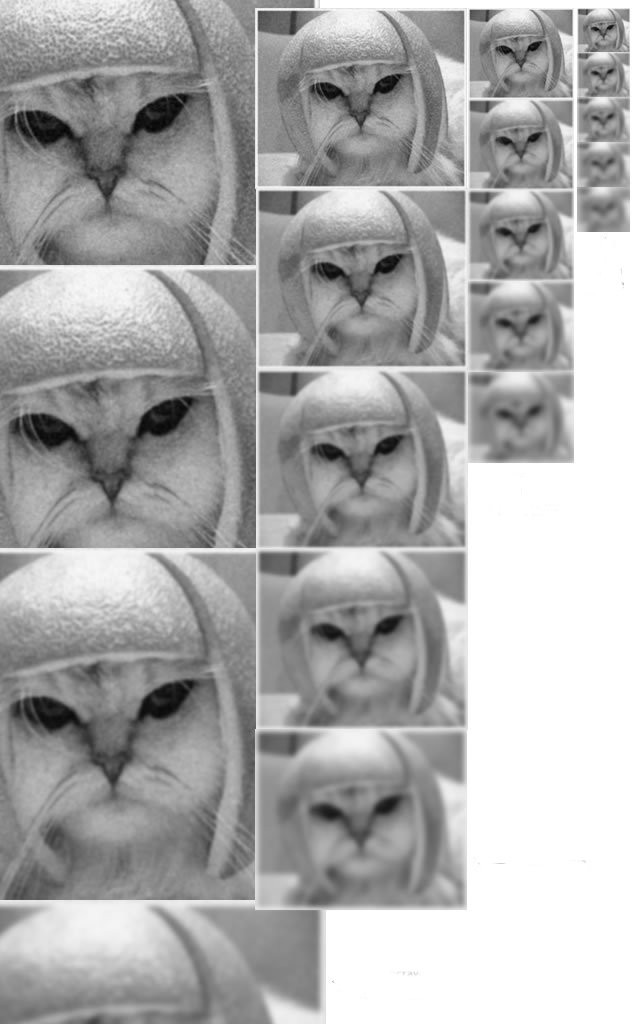
\includegraphics[width=0.8\textwidth]{pict/02/sift/sift_ais_octave.jpg}
\caption{Zestawienie kolejnych oktaw badanego obrazu.}
\label{fig:sift_ais_octave}
\end{figure}

\subsubsection{Różnica Gaussianów}
Kolejnym krokiem jest odjęcie od siebie sąsiadujących obrazów w oktawie. Uzyskane w ten sposób obrazy nazywamy różnicą Gausiannów (ang. DoG – Difference  of Gaussian). Z każdej 5 obrazowej oktawy otrzymujemy 4 obrazy różnicowe.
\begin{align}
D(x,y,\sigma) &= (G(x,y,k\sigma)-G(x,y,\sigma))*I(x,y)\\
&= L(x,y,k\sigma) - L(x,y,\sigma)
\end{align}

Różnica Gaussianów jest efektywną aproksymacją innej operacji służącej do lokalizowania punktów charakterystycznych – skalowo znormalizowanego Laplasianu Gausjanów $\sigma^2\nabla^2G$ (ang. LoG – Laplacian of Gaussian). Ekstrema LoG dostarczają znacznie bardziej stabilnych punktów charakterystycznych niż detektory takie jak Hessian czy funkcja Harrisa.
\begin{equation}
\frac{\partial G}{\partial \sigma}  = \sigma {\nabla}^2 G
\end{equation}
\begin{equation}
\sigma {\nabla}^2 G = \frac{\partial G}{\partial \sigma} \approx \frac{G(x,y,k\sigma)-G(x,y,\sigma)}{\sigma(k-1)}
\end{equation}

\begin{equation}
G(x,y,k\sigma)-G(x,y,\sigma) \approx (k-1)\sigma^2{\nabla}^2 G
\end{equation}
Aby obliczyć Laplasian Gausjanów należy obraz poddać rozmyciu, a następnie policzyć jego pochodne drugiego stopnia, aby znaleźć lokalne ekstrema. Rozmycie ma na celu redukcje szumów z obrazu, na które bardzo wrażliwe są pochodne drugiego stopnia. W efekcie otrzymujemy stabilne punkty reprezentujące krawędzie i narożniki w obrazie. Mankamentem tej metody jest złożoność obliczeniowa otrzymywania pochodnych drugiego stopnia. Stosując podejście zaproponowane w algorytmie SIFT, duży narzut operacji został zredukowany do prostej subtrakcji obrazów.
\begin{figure}[!htb]
\centering
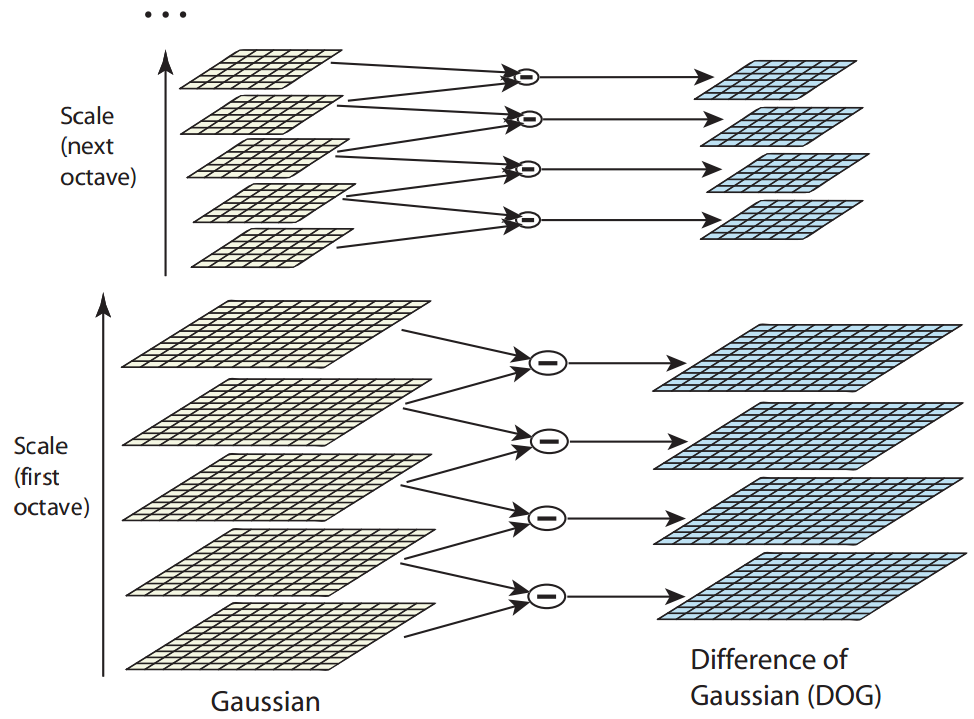
\includegraphics[width=0.8\textwidth]{pict/02/sift/sift_dgl_octave.png}
\caption{Schemat generowania obrazów różnicy Gaussianów}
\label{fig:sift_dgl_octave}
\end{figure}

%ZASTANOWIC SIE CZY COS NAPISAC O MULTIPLIKACJI
\subsubsection{Ekstrema jako potencjalne punkty charakterystyczne}
Aby zlokalizować lokalne ekstremum należy dokonać badania sąsiedztwa potencjalnego punktu charakterystycznego. W tym celu dokonujemy iteracji po wszystkich pikselach obrazu porównując je z otoczeniem "poziomym" (w obrębie jednego obrazu) jak i "pionowym" (czyli z otaczającymi pikselami z szeregu sąsiadujących rozmytych obrazów). Przedstawia to rysunek \ref{fig:sift_dgl_extremum}. W związku, że skrajne obrazy w oktawie mają tylko po jednym sąsiedzie, możemy je pominąć przy analizie.

\begin{figure}[!htb]
\centering
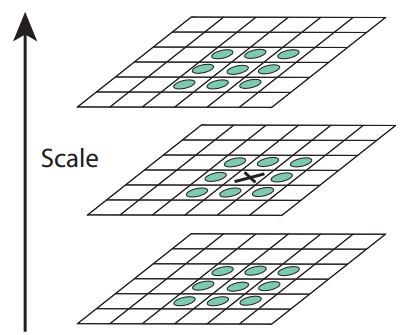
\includegraphics[scale=0.5]{pict/02/sift/sift_dgl_extremum.png}
\caption{Porównywanie otoczenia piksela w celu znalezienia lokalnego ekstremum}
\label{fig:sift_dgl_extremum}
\end{figure}
\subsubsection{Subpikselowa lokalizacja punktów charakterystycznych}
W związku, z tym, ekstrema często wypadają między sąsiadującymi pikselami, dokładną pozycję ekstremum uzyskuje się korzystając z rozwinięcia Taylora.
\begin{equation}
D(x) = D + \frac{\partial D^T}{\partial x}x + \frac{1}{2}x^T\frac{\partial^2D}{\partial x^2}x
\end{equation}

\begin{equation}
\widehat{x} = -\frac{\partial^2D}{\partial x^2}^{-1} \frac{\partial D}{\partial x}
\end{equation}




\subsection{Selekcja punktów charakterystycznych}
W wyniku działania wcześniej opisanych kroków algorytm generuję ogromną liczbę punktów charakterystycznych. Niestety znaczna część punktów jest słabej jakości, zbyt mało kontrastowa lub leży na krawędziach. Nie pozwala to na ich praktyczne wykorzystanie i takich punktów należy się pozbyć.
\subsubsection{Usuwanie cech mało kontrastowych}
Usuwanie cech mało kontrastowych odbywa się poprzez progowanie. Jeżeli wartość bezwzględna piksela obrazu DoG jest mniejsza niż heurystycznie dobrany próg piksel taki jest odrzucany. W pracy \cite{DGL04} autor algorytmu zakładał próg rzędu 3 \%. W przypadku gdy punktem charakterystycznym jest subpiksel, jego wartość podobnie jak pozycje wyliczamy z szeregu Taylora.
\begin{equation}
D(\widehat{x}) = D +   \frac{1}{2}\frac{\partial D}{\partial x}\widehat{x}
\end{equation}
\subsubsection{Usuwanie punktów lezących na krawędziach}
Różnica Gaussianów generuje silną odpowiedź na krawędziach. Powoduje to pewnego rodzaju przekłamania, jak np lokalizowanie punktów charakterystycznych w miejscach gdzie są one słabo określone i bardzo podatne na zakłócenia. 
W przypadku krawędzi, gradient prostopadły do niej jest duży, a równoległy mały. Warunki te nie są wystarczające do ulokowania stabilnego punktu charakterystycznego. Najlepsze punkty charakterystyczne znajdują się w rogach, ze względu na duże wartości gradientów w obu kierunkach.
W selekcji punktów charakterystycznych wykorzystuje się dwuwymiarową macierz Hesjanu \textbf{H}, która jest liczona w potencjalnym punkcie charakterystycznym i w skali jemu odpowiadającej.

\begin{equation}
\textbf{H} = 
\left[\begin{array}{cc}
D_{xx}&D_{xy}\\
D_{xy}&D_{yy}
\end{array}\right]
\end{equation}
Pochodne $D_{xx}$,$D_{yy}$,$D_{xy}$ są liczone poprzez odejmowanie pikseli z sąsiedztwa badanego punktu.


Wartości własne macierzy są proporcjonalne do głównej krzywizny obrazu różnicowego D. Na podstawie podejścia zaproponowanego przez Harrisa i Stephensona w 1988 roku \cite{HIS88}, obliczanie wartości własnych macierzy możemy zastąpić poprzez obliczenie ich stosunku. 

Niech $\alpha$ i $\beta$ będą wartościami własnymi macierzy. Ich sumę i iloczyn możemy obliczyć ze śladu i wyznacznika macierzy Hesjanu. 

\begin{equation}
Tr(\textbf{H}) = D_{xx} + D_{yy} = \alpha + \beta
\end{equation}

\begin{equation}
Det(\textbf{H}) = D_{xx} D_{yy} - {D_{xy}}^2 = \alpha  \beta
\end{equation}

Gdy wyznacznik macierzy \textbf{H} jest ujemny badany punkt jest odrzucany. W sytuacji gdy wyznacznik jest dodatni stosujemy podstawienie $\alpha = r \beta$ co pozwala nam zapisać stosunek między śladem i wyznacznikiem macierzy za pomocą samego współczynnika $r$
\begin{equation}
\frac{Tr(\textbf{H})^2}{Det(\textbf{H})} = \frac{(\alpha+\beta)^2}{\alpha\beta} = \frac{(r\beta+\beta)^2}{r\beta^2} = \frac{(r+1)^2}{r} 
\end{equation}
Aby wyeliminować odpowiedź krawędziową należy porównać stosunek głównych krzywizn badanego punktu i dokonać prostego progowania z użyciem współczynnika $r$.
 

\begin{equation}
\frac{Tr(\textbf{H})^2}{Det(\textbf{H})} < \frac{(r+1)^2}{r} 
\label{eqn:ratio_prog}
\end{equation}
Przedstawiona metoda jest bardzo efektywna obliczeniowo. Do przetestowania pojedynczego potencjalnego punktu charakterystycznego potrzebuje mniej niż 20 operacji zmiennoprzecinkowych. W badaniach \cite{DGL04} sugerowany współczynnik $r$ wynosi 10.


\subsection{Określenie orientacji punktów charakterystycznych}
Wyselekcjonowanego zbioru  punktów charakterystycznych należy przypisać orientacje. Zadanie to jest kluczowe w działaniu algorytmu, gdyż pozwala uniezależnić punkty charakterystyczne od rotacji obrazu. Na podstawie obrazu poddanemu rozmyciu Gaussa w skali rozmycia w jakiej dany punkt charakterystyczny został znaleziony wylicza się wartości i orientacje gradientów w otoczeniu punktu charakterystycznego:
\begin{equation}
m(x,y) = \sqrt{(L(x+1,y)-L(x-1,y))^2+(L(x,y+1)-L(x,y-1))^2}
\end{equation}
\begin{equation}
\theta(x,y) = atan(\frac{L(x,y+1)-L(x,y-1)}{L(x+1,y)-L(x-1,y)})
\end{equation}
\begin{figure}[!htb]
\centering
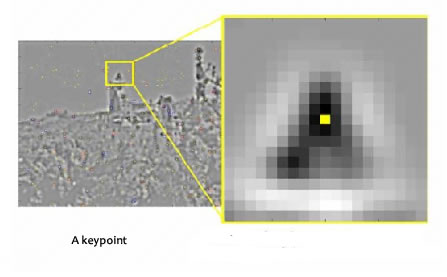
\includegraphics[width=0.8\textwidth]{pict/02/sift/sift_ais_orientation_1.jpg}
\caption{Badanie otoczenia punktu charakterystycznego - rozmycie}
\label{fig:sift_ais_orientation_1}
\end{figure}
\begin{figure}[!htb]
\centering
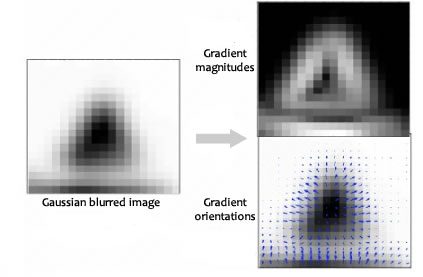
\includegraphics[width=0.8\textwidth]{pict/02/sift/sift_ais_orientation_2.jpg}
\caption{Badanie otoczenia punktu charakterystycznego - badanie gradientów}
\label{fig:sift_ais_orientation_2}
\end{figure}
W oparciu o rozkład gradientów wokół punktu charakterystycznego budowany jest histogram reprezentujący orientacje gradientów. Histogram ten jest podzielony 36 słupków o szerokości 10$^O$  pokrywający pełny zakres 360$^O$. Najwyższy pik wykresu odpowiada orientacji jaka zostanie przypisana punktowi charakterystycznemu. W sytuacji gdy inny słupek osiągnął wartość powyżej 80\% wartości maksymalnej, jego orientacja również zostaje odnotowana poprzez utworzenie dodatkowego bliźniaczego punktu, różniącego się orientacją. Według badań \cite{DGL04} tylko około 15\% posiada wielokierunkową orientacje, aczkolwiek jej uwzględnienie znacząco poprawia jakość dopasowań.
\begin{figure}[!htb]
\centering
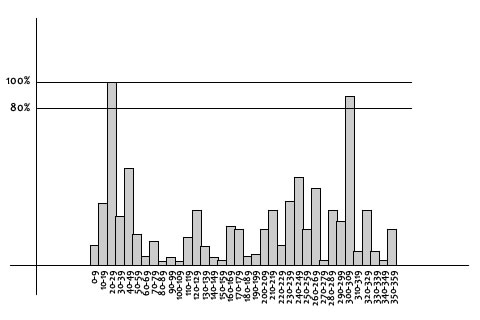
\includegraphics[width=0.8\textwidth]{pict/02/sift/sift_ais_orientation_histogram.jpg}
\caption{Histogram reprezentujący orientacje gradientów wokół punktu charakterystycznego}
\label{fig:sift_ais_orientation_histogram}
\end{figure}


\subsection{Budowa deskryptora}
Finalny etapem algorytmu SIFT jest wyliczenie  unikalnego deskryptora punktu charakterystycznego. Wokół punktu charakterystycznego badane jest okno o rozmiarze 16 na 16 pikseli podzielone na 16 sektorów. Sektor stanowi kwadrat o boku 4 pikseli. 
\begin{figure}[!htb]
\centering
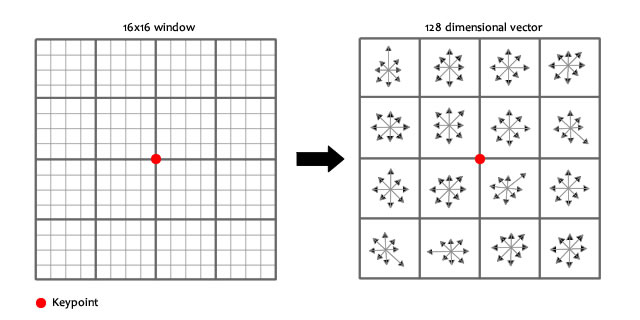
\includegraphics[width=0.8\textwidth]{pict/02/sift/sift_ais_16_16_128.jpg}
\caption{Tworzenie deskryptora punktu charakterystycznego - lokalna siatka histogramów}
\label{fig:sift_ais_16_16_128}
\end{figure}
Dla każdego pojedynczego sektora obliczane są wielkości i kierunki gradientów, które zostają zapisane za pomocą 8 wartościowego histogramu. Orientacje gradientów wyrażane są jako wielokrotności kąta 45$^O$.




\begin{figure}[!htb]
\centering
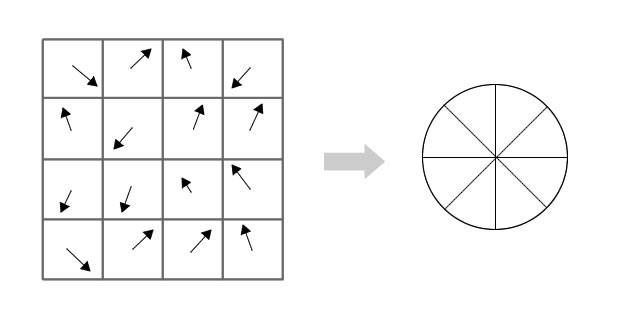
\includegraphics[width=0.8\textwidth]{pict/02/sift/sift_ais_4_4_8.jpg}
\caption{Tworzenie deskryptora punktu charakterystycznego - lokalna siatka histogramów}
\label{fig:sift_ais_4_4_8}
\end{figure}

Po obliczeniu 16 histogramów, cała tablica sektorów zostaje przeskalowana. Spowodowane to jest tym, że okna leżące bliżej punktu charakterystycznego są istotniejsze i należy im przypisać większa wagę. Analogicznie zmniejszany jest wpływ wartości znajdujących się brzegach badanego obszaru.

\begin{figure}[!htb]
\centering
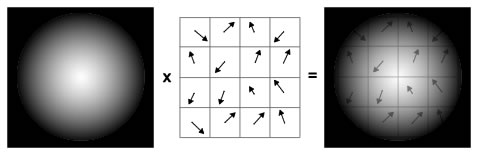
\includegraphics[width=0.8\textwidth]{pict/02/sift/sift_ais_des.jpg}
\caption{Siatka histogramów uwzględniająca odległość od punktu charakterystycznego}
\label{fig:sift_ais_des}
\end{figure}

W wyniku powyższych operacji otrzymujemy wektor 128 liczb (8-kierunkowe histogramy zgrupowane w 4 wierszach po 4 kolumny). Wektor ten jest poddawany normalizacji. 

Następnie aby uzyskać niezależność od rotacji, od wektora jest odejmowana orientacja punktu charakterystycznego obliczona w poprzednim etapie. Aby uzyskać niezależność od oświetlenia współczynniki znormalizowanego wektora, są poddawane półprogowaniu z parametrem 0,2. W sytuacji gdy jakiś współczynnik jest większy od zadanego progu, przypisywana mu jest wartość 0,2 po czym cały wektor poddawany jest ponownej normalizacji.

W wyniku całego procesu otrzymujemy 128 wymiarowy deskryptor punktu charakterystycznego.


%\begin{figure}[!htb]
%\centering
%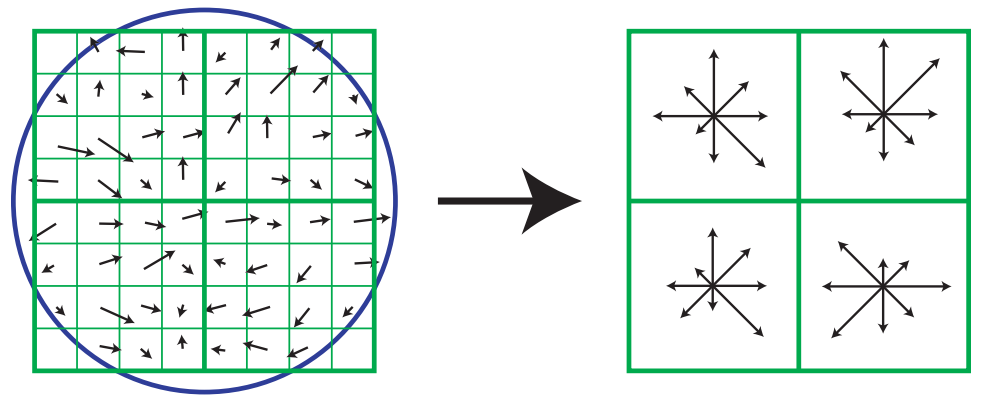
\includegraphics[width=0.8\textwidth]{pict/02/sift/sift/sift_dgl_keypoint.png}
%\caption{opis}
%\label{fig:sift_dgl_keypoint}
%\end{figure}

\FloatBarrier
\newpage
\section{Algorytm SURF}
Algorytm SURF (skrót od Speeded Up Robust Features) został po raz pierwszy zaprezentowany w 2006 roku w pracy doktorskiej Herberta Baya \cite{HB06}. Pełny jego opis można znaleźć również w pracy\cite{HB08}. Wykorzystywany jest on w zadaniach rozpoznawania obrazów oraz w rekonstrukcji obiektów trójwymiarowych. Algorytm częściowo jest inspirowany algorytmem SIFT i podobnie jak on aby usprawnić obliczenia korzysta z aproksymacji skomplikowanych operatorów. 

W jego działaniu możemy wyróżnić następujące etapy:
\begin{enumerate}
\item{Obliczenie obrazów całkowych.}
\item{Lokalizowanie punktów charakterystycznych.}
\item{Konstruowanie 64 wymiarowego deskryptora punktu charakterystycznego.}
\end{enumerate}
SURF podobnie jak algorytm SIFT jest chroniony patentem amerykańskim.
\subsection{Obliczenie obrazów całkowych}
Działanie algorytmu SURF rozpoczyna się od przygotowania obrazów całkowych. Są one wyliczane wg. wzoru \ref{eqn:surf_integral_images}.
\begin{equation}
I_{\sum}(x,y) = \sum\limits_{x'=0}^{ x} \sum\limits_{y'=0}^{y} I(x',y')
\label{eqn:surf_integral_images}
\end{equation}
Przygotowanie reprezentacji badanego obrazu w postaci całkowej pozwala, zredukować obliczenia intensywności dowolnego fragmentu obrazu do trzech prostych operacji arytmetycznych o stałym czasie wykonania. Ma to kluczowe znaczenie w przypadku analizy dużych fragmentów obrazów.


\begin{figure}[!htb]
\centering
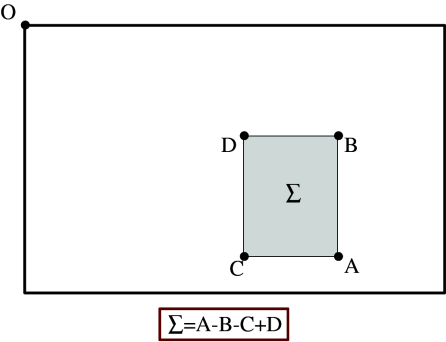
\includegraphics[width=0.8\textwidth]{pict/02/surf/surf_bay_integral_image.png}
\caption{Obliczanie intensywności wybranego obszaru w oparciu o obrazy całkowe}
\label{fig:surf_bay_integral_image}
\end{figure}



\subsection{Lokalizowanie punktów charakterystycznych}
\subsubsection{Wykrywanie punktów charakterystycznych za pomocą macierzy Hesjanu}
Algorytm do wykrywania obszarów charakterystycznych wykorzystuje macierz Hesjanu. Obszary te są lokowane w miejscach, w których wyznacznik macierzy osiąga lokalne maksimum.
\begin{equation}
\textbf{H}(x,y,\sigma) = 
\left[\begin{array}{cc}
L_{xx}(x,y,\sigma)&L_{xy}(x,y,\sigma)\\
L_{xy}(x,y,\sigma)&L_{yy}(y,y,\sigma)
\end{array}\right]
\end{equation}
Wyrażenie $L_{xx}(x,y,\sigma)$ to obraz splotu pochodnej cząstkowej drugiego stopnia funkcji rozmycia Gaussa ($D_{xx}=\frac{\partial^2}{\partial x^2}\frac{1}{2\pi\sigma^2}e^{-\frac{x^2+y^2}{2\sigma^2}}$) i obrazu I w punkcie (x,y). Analogicznie $L_{yy}(x,y,\sigma)$ i $L_{xz}(x,y,\sigma)$. Przedstawia je rysunek \ref{pict:surf_exact_kernel}

\begin{figure}
\centering
\subfigure[$D_{xx}$]{
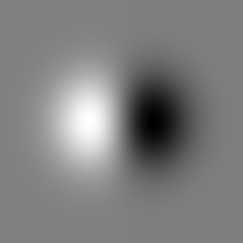
\includegraphics[scale=0.5]{pict/02/surf/dxx.png}}
\subfigure[$D_{yy}$]{
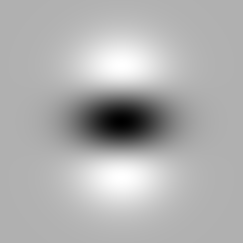
\includegraphics[scale=0.5]{pict/02/surf/dyy.png}}
\subfigure[$D_{xy}$]{
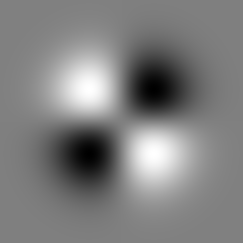
\includegraphics[scale=0.5]{pict/02/surf/dxy.png}}
\caption{Pochodne cząstkowe drugiego stopnia funkcji rozmycia Gaussa}
\label{pict:surf_exact_kernel}
\end{figure}
W praktyce stosuję się powyższe jądra w dyskretnej formie co przedstawia rysunek \ref{fig:surf_bay_gaussian_discretization}. Skutkuje to pogorszeniem jakości pracy operatorów w sytuacji gdy obraz jest obrócony o nieparzystą wielokrotność kąta $45^O$ i może prowadzić do pojawienia się artefaktów. 

\begin{figure}[!htb]
\centering
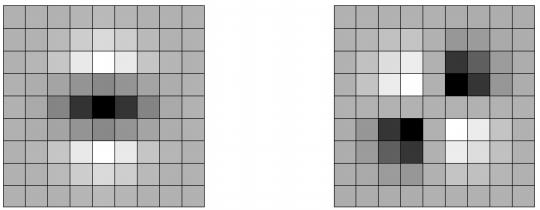
\includegraphics[width=0.8\textwidth]{pict/02/surf/surf_bay_gaussian_discretization.png}
\caption{Dyskretne pochodne cząstkowe drugiego stopnia Gaussianów}
\label{fig:surf_bay_gaussian_discretization}
\end{figure}
\subsubsection{Aproksymacja jąder rozmycia}
Bay podobnie jak Lowe w algorytmie SIFT zastosował podejście polegające na dużym uproszeniu realizowanych operacji. Jądra rozmycia zostały w radykalny sposób aproksymowane [rysunek \ref{fig:surf_bay_gaussian_approximation}].

\begin{figure}[!htb]
\centering
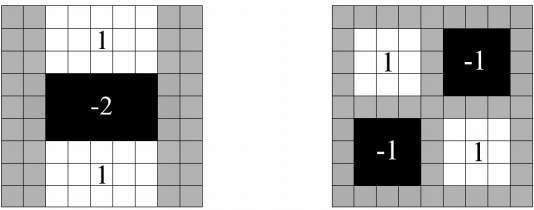
\includegraphics[width=0.8\textwidth]{pict/02/surf/surf_bay_gaussian_approximation.png}
\caption{Aproksymacje pochodnych cząstkowych drugiego stopnia Gaussianów}
\label{fig:surf_bay_gaussian_approximation}
\end{figure}

W związku z zastosowaniem aproksymowanych okien rozmycia wyrażenie na wyznacznik Hesjanu przyjmuje następująca postać:
\begin{equation}
det(\textbf{H}^{(a)}) = L_{xx}^{(a)} L_{yy}^{(a)}-(\omega L_{xy}^{(a)})^2
\label{eqn:det_aprox}
\end{equation}
Gdzie $L_{xx}^{(a)}$, $L_{yy}^{(a)}$, $L_{xy}^{(a)}$ to sploty obrazu I z aproksymowanymi oknami rozmycia, a współczynnik $\omega$ to waga potrzebna zachowania energii jąder Gaussowski przy korzystaniu z ich uproszczonej postaci. Obliczana jest ona według wyrażenia \ref{eqn:frobo}, gdzie $\|\|_F$ oznacza normę Frobeniusa.


\begin{equation}
\omega = \frac{\|L_{xy}(\sigma)\|_F\|D_{yy}(rozmiar-okna)\|_F}{\|L_{yy}(\sigma)\|_F\|D_{xy}(rozmiar-okna)\|_F}
\label{eqn:frobo}
\end{equation}
Dla okna rozmycia $\sigma=1.2$ o wymiarach $9\times9$ współczynnik $\omega$ wynosi:
\begin{equation}
\omega = \frac{\|L_{xy}(1.2)\|_F\|D_{yy}(9)\|_F}{\|L_{1.2}(\sigma)\|_F\|D_{xy}(9)\|_F} = 0.9127\simeq0.9
\end{equation}
Teoretycznie każdemu rozmyciu i rozmiarowi okna odpowiada inna wartość wagi $\omega$. Praktyka jednak pokazuje, że dla usprawnienia pracy algorytmu możemy $\omega$ traktować jaką stałą, bez dużej straty dokładności. 

 W sposób znaczny przyśpiesza to obliczenia, a jak wykazały badania \cite{HB06} nie tylko nie pogarsza to wyników, a wręcz je polepsza [rysunek \ref{fig:surf_bay_compare_fast}].




\begin{figure}[!htb]
\centering
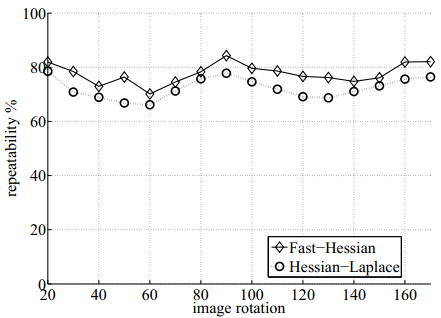
\includegraphics[scale=0.8]{pict/02/surf/surf_bay_compare_fast.png}
\caption{Porównanie działania operatorów dokładnych i aproksymowanych w zależności od kąta rotacji obrazu}
\label{fig:surf_bay_compare_fast}
\end{figure}

\subsubsection{Skalo-przestrzenna reprezentacja obrazu}
Lokalizowanie punktów kluczowych odbywa się w różnych skalach obrazu. Obrazy skalo-przestrzenne są najczęściej reprezentowane w postaci piramidy obrazów. Kolejne obrazy są poddawane progresywnemu rozmyciu oraz podpróbkowaniu, tworząc oktawy.
\begin{figure}[!htb]
\centering
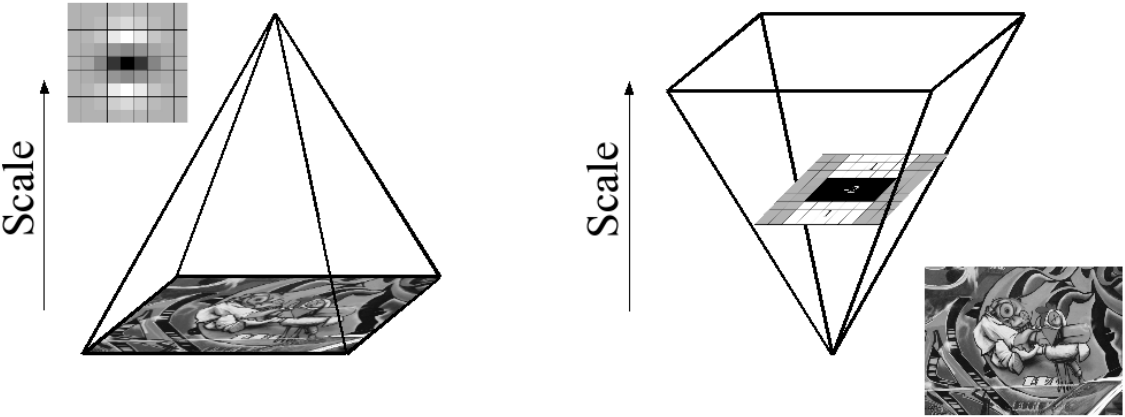
\includegraphics[width=0.8\textwidth]{pict/02/surf/surf_bay_scale_piramid.png}
\caption{Piramida skalo-przestrzenna}
\label{fig:surf_bay_scale_piramid}
\end{figure}


Dzięki zastosowaniu obrazów całkowych i błyskawicznie skalowalnych okien rozmycia, operacje skalo-przestrzenne dają się w łatwy sposób zrównoleglić.



\subsubsection{Skalowanie jąder rozmycia}
\begin{figure}[!htb]
\centering
\subfigure[$D_{yy}$]{
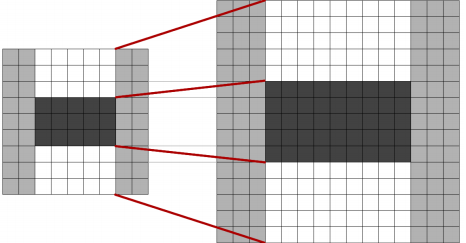
\includegraphics[scale=0.62]{pict/02/surf/surf_bay_prescale_gaussian_1.png}}
\subfigure[$D_{xy}$]{
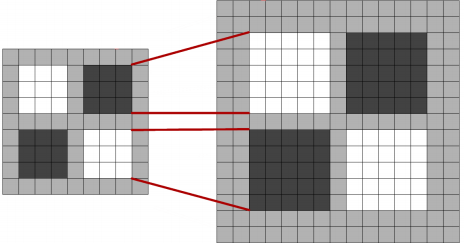
\includegraphics[scale=0.62]{pict/02/surf/surf_bay_prescale_gaussian_2.png}}
\caption{Przeskalowane okna rozmycia}
\label{fig:surf_bay_prescale_gaussian}
\end{figure}
Każde okno rozmycia jest kwadratem o boku $3l$ które można opisać za pomocą następujących wyrażeń:

\begin{align}
 l &= 2^oi+1\\
\label{eqn:liczym_l}
\end{align}
gdzie:

{\centering
\begin{tabular}{cclll}
o & - &  numer oktawy     &&$o=1,2,3,4,...$\\ 
i & - & stopień rozmycia w oktawie &&$i=1,2,3,4$\\ 
\end{tabular} 
}


W związku z powyższym wzór na odchylenie standardowe rozmycia Gaussa $\sigma$ możemy zapisać:

\begin{align}
\sigma &= \frac{1.2}{3}l\\
\label{eqn:sigma_o_i_l}
\end{align}


\begin{equation}
D_{xx} = \left\lbrace \begin{array}{ccl}
-2&&  (x,y) \in [-\frac{l}{2},\frac{l}{2}]\times]-l,l[\\
+1&&  (x,y) \in [-\frac{l}{2},\frac{l}{2}]\times]-l,l[\times[-\frac{3l}{2},\frac{3l}{2}]\setminus]-l,l[ \\
0 && reszta
\end{array} \right.
\end{equation}

\begin{equation}
D_{yy} = \left\lbrace \begin{array}{ccl}
-2&&  (x,y) \in ]-l,l[\times[-\frac{l}{2},\frac{l}{2}]\\
+1&&  (x,y) \in ]-l,l[\times[-\frac{3l}{2},\frac{3l}{2}]\setminus]-l,l[\times[-\frac{l}{2},\frac{l}{2}] \\
0 && reszta 
\end{array} \right.
\end{equation}

\begin{equation}
D_{xy} = \left\lbrace \begin{array}{ccl}
+1&&  (x,y) \in ]0,-l]\times]0,+l]\bigcap]0,+l]\times[-l,0[ \\
-1&&  (x,y) \in [-l,0[\times[-l,0[\bigcap]0,+l]\times]0,+l]\\
0 && reszta
\end{array} \right.
\end{equation}




\begin{equation}
\sigma^2=\frac{L^2-1}{12}
\label{eqn:sigma_2_L}
\end{equation}


 

\begin{figure}[!htb]
\centering
\subfigure[$D_{yy}$]{
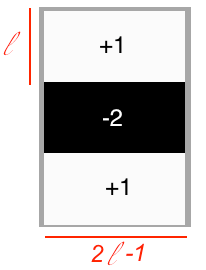
\includegraphics[scale=1]{pict/02/surf/dyy_prescale.png}}
\subfigure[$D_{xy}$]{
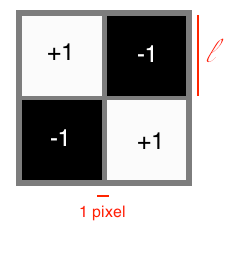
\includegraphics[scale=1]{pict/02/surf/dxy_prescale.png}}
\caption{Okna rozmycia}
\label{fig:surf_bay_prescale_gaussian_3}
\end{figure}

\begin{table}
\centering

\begin{tabular}{|c|c|c|c|c|c|c|}
  \hline 
   o & i & $\sigma$ & l & L & $\lambda$ & $\omega$ \\ 
  \hline 
   1 & 1 & 1,2 & 3 & 4,275 & 2 & 0,9127 \\ 
  \hline 
     & 2 & 2,0 & 5 & 7,000 & 4 & 0,9487 \\ 
  \hline 
     & 3 & 2,8 & 7 & 9,751 & 6 & 0,9636 \\ 
  \hline 
     & 4 & 3,6 & 9 & 12,511 & 7 & 0,9718 \\ 
  \hline 
   2 & 1 & 2,0 &5 & 8,000 & 4 & 0,9487 \\ 
  \hline 
     & 2 & 3,6 & 9 & 12,510 & 7 & 0,9718 \\ 
  \hline 
     & 3 & 5,2 & 13 & 18,041 & 10 & 0,9806 \\ 
  \hline 
     & 4 & 6,8 &17 & 23,577 & 14 & 0,9852 \\ 
  \hline 
   3 & 1 & 3,6 & 9 & 12,510 & 7 & 0,9718 \\ 
  \hline 
     & 2 & 6,8 & 17 & 23,577 & 14 & 0,9852 \\ 
  \hline 
     & 3 & 10,0 & 25 & 34,655 & 20 & 0,9900 \\ 
  \hline 
    & 4 &13,2 & 33 & 45,737 & 26 & 0,9924 \\ 
  \hline 
   4 & 1& 6,8 & 17 & 23,577 & 14 & 0,9852 \\ 
  \hline 
    & 2 &13,2 & 33 & 45,737 & 26 & 0,9924 \\ 
  \hline 
    & 3 &19,6 & 49 & 67,903 & 39 & 0,9949 \\ 
  \hline 
    & 4 &26,0 & 65 & 90,072 & 52 & 0,9962 \\ 
  \hline 
  \end{tabular}
  \caption{Wartości charakterystyczne dla okien aproksymowanych filtrów rozmycia}
  \label{tab:surf_parameters}
\end{table}

\begin{figure}[!htb]
\centering
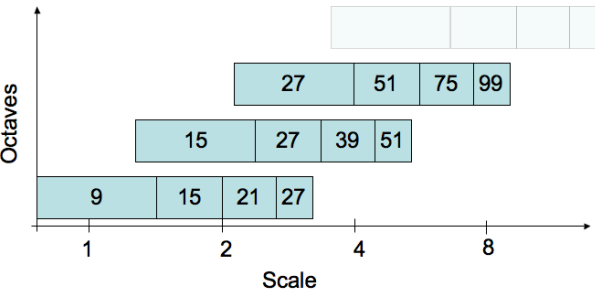
\includegraphics[width=0.8\textwidth]{pict/02/surf/surf_bay_octave_scale.png}
\caption{Rozmiar okna filtru w zależności od oktawy i stopnia rozmycia}
\label{fig:surf_bay_octave_scale}
\end{figure}
Tabela \ref{tab:surf_parameters} przedstawia charakterystyczne parametry filtrów. Zostały w niej przedstawione właściwości dla 4 pierwszych oktaw. Algorytm zakłada możliwość analizowania większej ilości oktaw. Ich parametry są obliczane w analogiczny sposób, dopóki okno filtru nie przekracza rozmiaru obrazu. W praktyce jednak badania najczęściej ogranicza się do 4 pierwszych oktaw, gdyż ze wzrostem skali znacząco spada liczba lokalizowanych punktów charakterystycznych [wykres \ref{fig:surf_bay_scale_histogram}].


\begin{figure}[!htb]
\centering
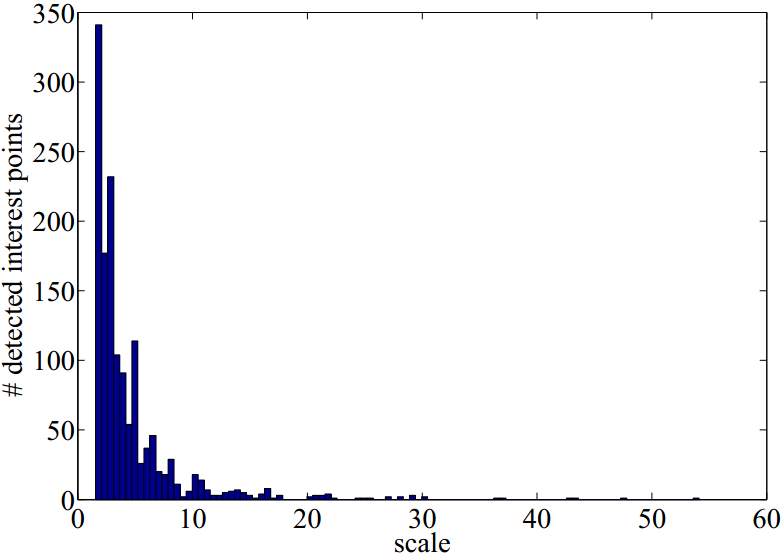
\includegraphics[scale=0.7]{pict/02/surf/surf_bay_scale_histogram.png}
\caption{Ilość lokalizowanych punktów charakterystycznych w zależności od skali}
\label{fig:surf_bay_scale_histogram}
\end{figure}










\subsection{Określenie orientacji punktów charakterystycznych}
Do określenia orientacji punktu charakterystycznego wykorzystywana jest falka Haara. Dla pikseli znajdujących się w otoczeniu punktu charakterystycznego liczone są odpowiedzi falki Haara w kierunku poziomym i pionowym. Poprzez otoczenie rozumiany jest kołowy obszar o promieniu $6\sigma$, gdzie $\sigma$ odpowiada skali w jakiej został zlokalizowany punkt. Podobnie rozmiar falki zależy od skali. Do jej liczenia wykorzystujemy okno o boku $4\sigma$. Dzięki zastosowaniu przygotowanych wcześniej obrazów całkowych liczba operacji potrzebnych do policzenia odpowiedzi w jednym kierunku została zredukowana do 6.


Odpowiedzi falek są reprezentowane na układzie współrzędnych. Oś OX reprezentuje odpowiedzi poziome, OY pionowe, a punkt przecięcia stanowi punkt charakterystyczny. Następnie wykorzystując obracające się wokół początku układu współrzędnych okno będące wycinkiem koła o kącie $\frac{\pi}{3}$. Odpowiedzi znajdujące się wewnątrz okna są sumowane. Suma odpowiedzi stanowi długość wektora związanego z kątem w jakim znajduje się okno. Kąt orientacji punktu charakterystycznego jest kątem w którym długość wektora sum odpowiedzi jest największa [rys.\ref{fig:surf_bay_orientation_assignment_c}].

\begin{figure}[!htb]
\centering
\subfigure[]{
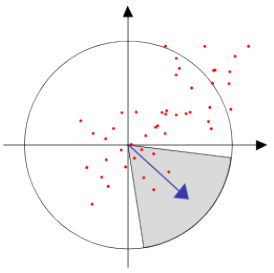
\includegraphics[scale=0.6]{pict/02/surf/surf_bay_orientation_assignment_1.png}}
\subfigure[]{
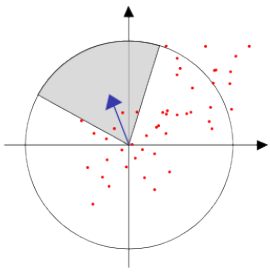
\includegraphics[scale=0.6]{pict/02/surf/surf_bay_orientation_assignment_2.png}}
\subfigure[]{
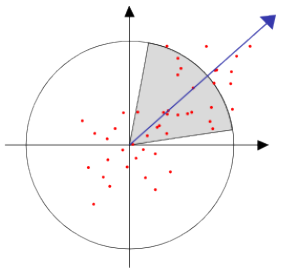
\includegraphics[scale=0.6]{pict/02/surf/surf_bay_orientation_assignment_3.png}
\label{fig:surf_bay_orientation_assignment_c}}

\caption{Badanie orientacji punktu charakterystycznego}
\label{fig:surf_bay_orientation_assignment}
\end{figure}


\subsection{Budowa deskryptora}
Podobnie jak algorytm SIFT, SURF do budowy deskryptora wykorzystuje informacje o otoczeniu punktu charakterystycznego. Wokół badanego punktu analizowany jest kwadratowy obszar o boku $20\sigma$. 

Okno to jest zorientowanie zgodnie z kierunkiem wyznaczonym w poprzednim kroku i podzielone na 16 regularnych subregionów. Każdy subregion jest w równych odstępach próbkowany w efekcie czego otrzymujemy zbiór $5\times5$ pikseli. Dla wycinka reprezentującego subregion liczona jest falka Haara w kierunku równoległym i normalnym do orientacji punktu charakterystycznego.  Falka ta ma rozmiar $2\sigma$ W praktyce aby zwiększyć szybkość działania algorytmu falki są liczone dla nie obróconego obrazu, a następnie ich odpowiedzi są interpolowane do kierunku rotacji. 
\begin{figure}[!htb]
\centering
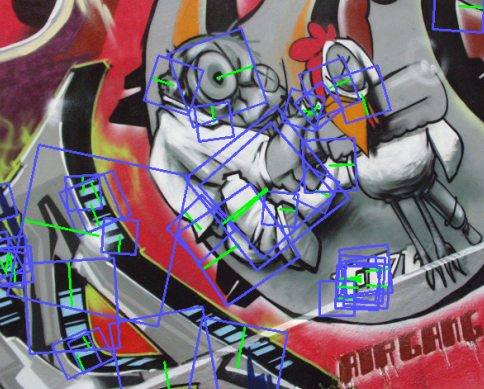
\includegraphics[scale=0.8]{pict/02/surf/surf_bay_example.png}
\caption{Badane obszary charakterystyczne}
\label{fig:surf_bay_example}
\end{figure}
W celu minimalizacji błędów spowodowanych geometrycznymi deformacjami odpowiedzi falek $d_x$ i $d_y$ są normalizowane rozkładem Gaussa z rozkładem równym $3.3\sigma$ (gdzie $\sigma$ oznacza skale w jakiej badany jest obszar).

\begin{figure}[!htb]
\centering
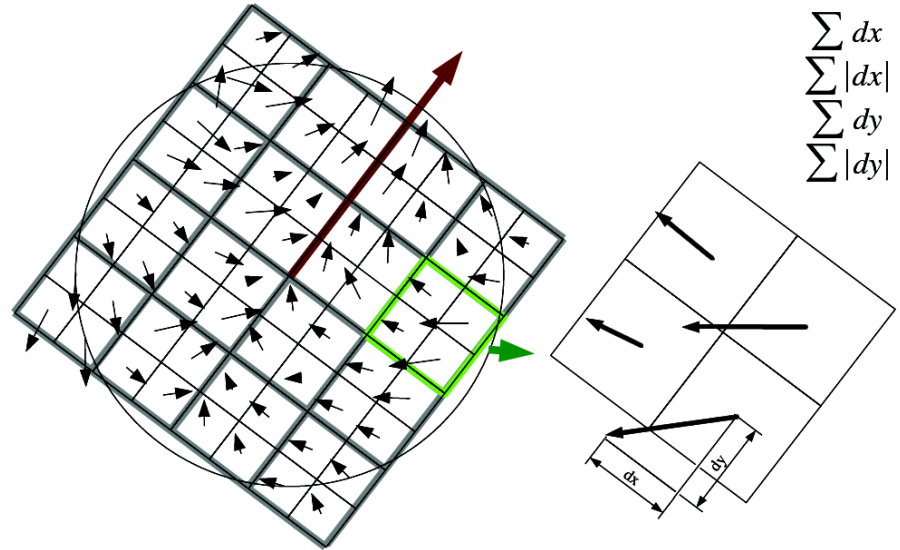
\includegraphics[width=0.8\textwidth]{pict/02/surf/surf_bay_scale_descriptor.png}
\caption{Badanie otoczenia punktu charakterystycznego}
\label{fig:surf_bay_scale_descriptor}
\end{figure}

Falki w obrębie jednego subregionu są sumowane. Ponadto sumowaniu poddane są wartości bezwzględne falek. Zabieg ten ma na celu pozyskanie informacji o biegunowości intensywności zmian. W wyniku tych działań otrzymujemy 4 wymiarowy wektor opisujący subregion.

\begin{equation}
v_{subregion} = \left[ \sum d_x,\sum d_y,\sum |d_x|,\sum |d_y|\right] 
\end{equation}

\begin{figure}[!htb]
\centering
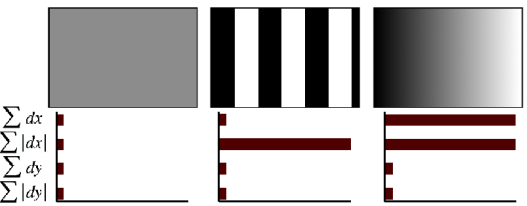
\includegraphics[width=0.8\textwidth]{pict/02/surf/surf_bay_gradient.png}
\caption{Przykłady wektorów opisujących subregiony w zależności od natury obszaru charakterystycznego}
\label{fig:surf_bay_gradient}
\end{figure}

W skład deskryptora punktu charakterystycznego wchodzi 16 subregionów w efekcie czego otrzymujemy 64 wymiarowy wektor punktu charakterystycznego. Algorytmu posiada wariacje różniące się rozdzielczością na jaką jest podzielony badany obszar charakterystyczny. Badania \cite{HB08} wykazują jednak 64 wymiarowy deskryptor jest rozwiązaniem najlepszym i optymalnym [\ref{fig:surf_bay_compare}]. W sytuacji, w której lekki spadek jakości jest akceptowalny na rzecz znaczącej poprawy czasu dopasowywania punktów charakterystycznych, wartym rozważenia jest deskryptor SURF-36 ($3\times3\times4$)
\begin{figure}[!htb]
\centering
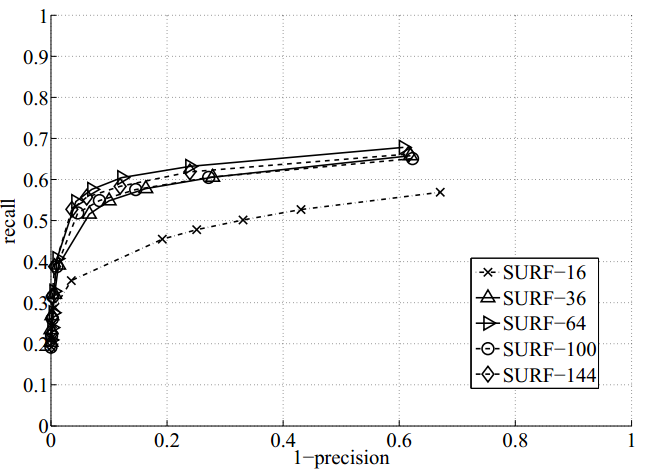
\includegraphics[width=0.8\textwidth]{pict/02/surf/surf_bay_compare_dim.png}
\caption{Porównanie deskryptorów SURF}
\label{fig:surf_bay_compare}
\end{figure}


Otrzymany deskryptor dzięki zastosowaniu falek jest niezależny od rotacji,skali, zmiennego  oświetlenia. Po normalizacji do wektora jednostkowego uzyskuje ponadto niezależność od kontrastu. Co więcej dzięki zastosowaniu całkowania informacji gradientach w subregionach, algorytm SURF jest również bardziej odporny na zaszumienie obrazu niż algorytm SIFT [rys. \ref{fig:surf_bay_clean_noisy}]. 
\begin{figure}[!htb]
\centering
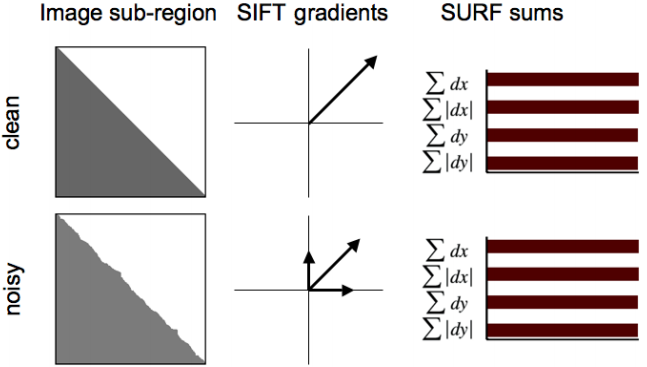
\includegraphics[width=0.8\textwidth]{pict/02/surf/surf_bay_clean_noisy.png}
\caption{Wpływ szumu na wygląd deskryptorów subregionów algorytmów SIFT i SURF}
\label{fig:surf_bay_clean_noisy}
\end{figure}
\FloatBarrier
\newpage
\section{Algorytm STAR}
Algorytm STAR to zoptymalizowany algorytm {CenSurE} (skr. Center Surround Extremas) \cite{CENS} rozwijany w laboratorium robotyki Willow Garrage. Stanowi rozwinięcie podejścia zastosowanego w  algorytmie SURF. 


\subsection{Obliczenie pochyłych obrazów całkowych}

Algorytm STAR podobnie jak SURF korzysta z obrazów całkowych. Raz obliczona reprezentacja obrazu może być wielokrotnie wykorzystywana w trakcie analizy. W sposób znaczący przyśpiesza to prace algorytmu i zapewnia stały czas wykonywania operacji niezależnie od rozmiaru badanego obszaru. Ze względu na użycie w algorytmie STAR filtrów o skomplikowanych kształtach modyfikacji uległa funkcja obliczająca obrazy. Zamiast stosowanego w SURF wzoru:
\begin{equation}
I_{\sum}(x,y) = \sum\limits_{x'=0}^{ x} \sum\limits_{y'=0}^{y} I(x',y')
\label{eqn:star_integral_images_old}
\end{equation}
obrazy całkowe w algorytmie STAR obliczane są według następującej formuły:
\begin{equation}
I_{\sum\alpha}(x,y) = \sum\limits_{y'=0}^{ y} \sum\limits_{x'=0}^{x+\alpha(y-y')} I(x',y')
\label{eqn:star_integral_images}
\end{equation}
gdzie $\alpha$ jest stałą zależną od rodzaju stosowanego filtru. Gdy $\alpha=0$ wzór \ref{eqn:star_integral_images} przyjmuje postać wzoru \ref{eqn:star_integral_images_old}. Gdy $\alpha>0$ obszar obrazu całkowego jest pochylony w prawo (jak na rysunku \ref{fig:cs_trapezoidal}), a gdy $\alpha<0$ w lewo. 

\begin{figure}
\centering
\subfigure[]{
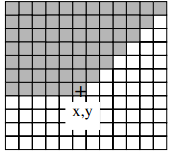
\includegraphics[scale=0.8]{pict/02/star/cs_integral_image_a.png}}
\subfigure[]{
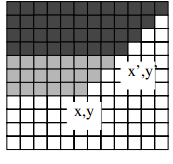
\includegraphics[scale=0.8]{pict/02/star/cs_integral_image_b.png}}
\caption{Przykład zastosowania pochyłych obrazów całkowych dla trapezoidalnego obszaru}
\label{fig:cs_trapezoidal}
\end{figure}







\subsection{Lokalizowanie punktów charakterystycznych}


Do lokalizowania punktów charakterystycznych algorytm STAR wykorzystuje dwustopniowe filtry otoczeniowo-centryczne, stanowiące łatwą i szybką w obliczeniach aproksymacje Laplasjanu. W STAR zastosowano inspirowany falkami Haara dwustopniowy filtr otoczeniowo-centryczny [rys. \ref{fig:star_bi_filters}].



\begin{figure}[!htb]
\centering
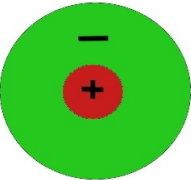
\includegraphics[scale=0.5]{pict/02/star/wg_haar.png}
\caption{Schemat dwustopniowego filtru otoczeniowo-centrycznego}
\label{fig:wg_haar}
\end{figure}

\subsubsection{Dwustopniowe filtry otoczeniowo-centryczne}

W ramach prac nad algorytmem {CenSurE} przetestowano szereg dwustopniowych filtrów począwszy od kołowego operatora LoG po dwustopniowy filtr kwadratowy. Filtr kołowy jest najwierniejszą reprezentacją Laplasjanu, aczkolwiek jest najbardziej złożony obliczeniowo. Bardzo szybkie filtry kwadratowe są z kolei podatne na rotacje obrazu i ich efektywność spada przy obrotach o nieparzyste wielokrotności kąta $45^O$. Odpowiedni filtr powinien być kompromisem między liczbą stopni symetrii i złożonością obliczeniową. W algorytmie {CenSurE} zastosowano filtr ośmiokątny [rys. \ref{fig:cs_okt}] dający się łatwo obliczać dzięki zastosowaniu pochyłych obrazów całkowych. Optymalizując algorytm {CenSurE} wypracowano rozwiązanie złożone 2 obróconych względem siebie o kąt $45^O$ kwadratów [rys. \ref{fig:wg_circle_aprox}] tworzących gwiazdę - skąd nazwa algorytm STAR (w tłumaczeniu z angielskiego "gwiazda").



\begin{figure}[!htb]
\centering
\subfigure[]{
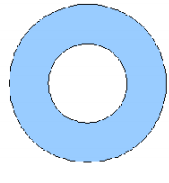
\includegraphics[height=25mm]{pict/02/star/cs_circle_aprox_a.png}
}
\subfigure[]{
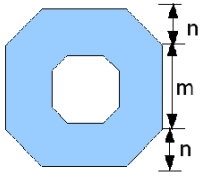
\includegraphics[height=25mm]{pict/02/star/cs_circle_aprox_b.png}
\label{fig:cs_okt}
}
\subfigure[]{

\includegraphics[height=25mm]{pict/02/star/cs_circle_aprox_c.png}
}
\subfigure[]{
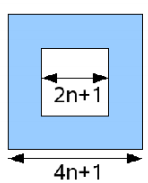
\includegraphics[height=25mm]{pict/02/star/cs_circle_aprox_d.png}
}
\caption{Dwustopniowe filtry otoczeniowo-centryczne}
\label{fig:star_bi_filters}
\end{figure}


\begin{figure}
\centering
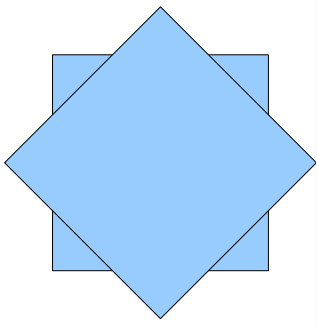
\includegraphics[height=35mm]{pict/02/star/wg_circle_aprox.png}
\caption{Dwustopniowy filtr otoczeniowo-centryczny wykorzystywany w algorytmie STAR}
\label{fig:wg_circle_aprox}
\end{figure}

Zastosowanie 2 okien o jednakowej powierzchni wyeliminowało problem równoważenia odpowiedzi dodatnich i ujemnych, oraz znacznie uprościło obliczenia. Podobnie jak w algorytmie SURF aby zwiększyć skale w jakiej lokalizujemy punkt charakterystyczny należy zwiększyć rozmiar filtra. 

\subsubsection{Ekstrema jako potencjalne punkty charakterystyczne}

Dla pojedynczego piksela obrazu jest liczone 7 odpowiedzi falek otoczeniowo-centrycznych o różnych rozmiarach. Każda falka reprezentuje obraz w innej skali. Algorytm dopuszcza liczenie większej ilości filtrów, aczkolwiek do większości zastosowań 7 okien jest liczbą wystarczającą.

Po obliczeniu odpowiedzi lokalizowane są lokalne ekstrema. Wartości falek są porównywane w pionowym i poziomym otoczeniu podobnie jak w omówionych wcześniej algorytmach. Jako potencjalne punkty charakterystyczne wybierane są piksele, które w swoim sąsiedztwie osiągają wartości ekstremalne. 

\subsection{Selekcja punktów charakterystycznych}
\subsubsection{Eliminacja słabych punktów}
Wartość bezwzględna odpowiedzi filtru dostarcza informacji o jakości punktu charakterystycznego. Im wartość ta jest większa tym punkt jest bardziej powtarzalny. W celu poprawy stabilności lokalizowanych dokonuje się progowania i odrzuca punkty o małej wartości bezwzględnej.
\subsubsection{Usuwanie punktów lezących na krawędziach}
Jak zostało opisane przy omawianiu algorytmu SIFT aby wybrać najbardziej stabilne cechy obrazu ze zbioru punktów charakterystycznych należy usunąć punkty leżące na krawędziach.W odróżnieniu do algorytmów SIFT i SURF, w algorytmie STAR zamiast macierzy Hesjanu użyto miary Harrisa.

\begin{equation}
\textbf{H} = 
\left[\begin{array}{cc}
\sum L_{x}^2&\sum L_{x}L_{y}\\
\sum L_{x}L_{y}&\sum L_{y}^2
\end{array}\right]
\end{equation}
$L_{x}$ i $L_{y}$ są pochodnymi funkcji filtru w kierunkach x i y, a sumowanie odbywa się w obrębie okna w jakim punkt charakterystyczny został zlokalizowany.


Dalsza część postępowanie jest analogiczna jak we wspomnianym algorytmie SIFT. Badany jest wyznacznik i ślad macierzy na podstawie których określa się współczynnik głównych krzywizn. W oparciu o obliczony współczynnik piksele poddawane są progowaniu [wzór \ref{eqn:ratio_prog}]. Domyślna wartość progu wynosi 10.


\subsection{Budowa deskryptora}
Algorytm STAR jest detektorem punktów charakterystycznych. Nie posiada on własnego mechanizmu opisu cech. Aby móc go stosować należy go połączyć, z algorytmem deskrypcyjnym takim jak np. deskryptor SIFT lub SURF. W raporcie dotyczącym badań nad algorytmem CenSurE autorzy posługują się zmodyfikowanym deskryptorem SURF. 




\FloatBarrier
\newpage
\section{Algorytm FAST}
Algorytm FAST (skr. Features from Accelerated Segment Test) został opublikowany przez Edwarda Rostena i Toma Drummonda w 2006 roku \cite{rosten_2006_machine} \cite{rosten_2008_faster}.  Algorytm ten służy do lokalizowania rogów w obrazie, które mogą być wykorzystane do zadań rozpoznawania i śledzenia. 

W odróżnieniu do wcześniej omawianych algorytmów FAST nie dokonuje "globalnej" analizy obrazu w poszukiwaniu cech charakterystycznych. Wykorzystując algorytmy uczenia maszynowego bada małe wycinki obrazu.

FAST nie dokonuje wieloskalowego poszukiwania punktów charakterystycznych. Chcąc osiągnąć niezależność od skali z oryginalnego obrazu należy wygenerować piramidę skalową, czyli zbiór obrazów reprezentujących widoki w różnych skalach.

\subsection{Zasady egzaminowania}
Jak wspomniano we wstępie, algorytm FAST należy do grupy algorytmów badających indywidualnie segmenty obrazu. Segment stanowi punkt $p$ i utworzony wokół niego okrąg składający się z 16 pikseli [rys. \ref{fig:fast_test_segment}]. 

Punkt $p$ jest uznawany jako róg jeżeli istnieje zbiór $n$ sąsiadujących pikseli okręgu, które są jaśniejsze od  intensywności punktu $p$ powiększonej o wartość progu $t$ ($I_p + t$), lub ciemniejsze od intensywności punktu $p$ pomniejszonej o próg $t$ ($I_p - t$). 

Jako wartość $n$ najczęściej przyjmuje się liczbę 12. W praktyce badanie punktu rozpoczyna się od zbadania 4 pikseli umieszczonych w głównych osiach punktu $p$. Dla rysunku \ref{fig:fast_test_segment} są to piksele 1,5,9,13. Jeżeli punkt $p$ jest rogiem, wówczas co najmniej 3 z 4 egzaminowanych pikseli muszą być jaśniejsze niż $I_p + t$ lub ciemniejsze niż $I_p - t$. Test ten pozwala w szybki sposób wykluczyć dużą liczbę punktów. Dla pozostałych punktów, które przeszły przez wstępny proces selekcji, badane są wszystkie piksele w otaczającym je segmencie.

Przytoczona metoda cechuję się dużą wydajnością, aczkolwiek jej autorzy zwracają uwagę na następujące wady:
\begin{enumerate}
\item Aby móc skutecznie zastosować szybki test wstępny 4 pikseli $n$ musi wynosić 12.
\item Wybór i kolejność testowania 4 pikseli w szybkim teście wpływa na rozkład lokalizowania punktów. Wada ta nabiera znaczenie przy zastosowaniach w czasie rzeczywistym.
\item Informacje uzyskane w szybkim teście 4 pikseli są niewykorzystywane przy dokładnym badaniu punktu.
\item Metoda może lokalizować wiele punków stykających się ze sobą.
\end{enumerate}



\begin{figure}[!htb]
\centering
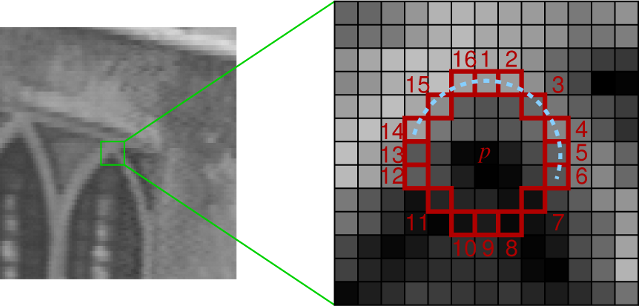
\includegraphics[width=0.8\textwidth]{pict/02/fast/fast_test_segment.png}
\caption{Badanie otoczenia punktu potencjalnego rogu}
\label{fig:fast_test_segment}
\end{figure}





\subsection{Uczenie maszynowe}
Algorytm FAST w swoim działaniu wykorzystuje metody uczenia maszynowego. Proces ten jest podzielony na dwa etapy:
\begin{enumerate}
\item budowa detektora rogów
\item budowa drzewa decyzyjnego
\end{enumerate}


W pierwszym etapie na podstawie zbioru uczącego jest budowany detektor rogów. Algorytm bada wszystkie pikseli wchodzące w skład obrazu uczącego z zastosowaniem testów segmentowych. Używane testy są wolne, gdyż na tym etapie egzaminowane są wszystkie 16 pikseli wchodzące w skład pojedynczego segmentu.

Wszystkie piksele w okręgu $x\in{1,2,3,...,16}$ są klasyfikowane względem jasności punktu $p$. Mogą się one znajdować w 3 stanach:

\begin{equation}
S_{p\rightarrow x} = 
\left\lbrace\begin{array}{cccccccccc}
$d,$ & & &            &      & I_{p\rightarrow x} & \leq & I_{p} - t   &  $(ciemniejszy)$  \\
$s,$ & & & I_{p} - t  & <    & I_{p\rightarrow x} & <    & I_{p} + t   &  $(podobny)$  \\
$b,$ & & & I_{p} + t  & \leq & I_{p\rightarrow x} &      &             &  $(jaśniejszy)$  \\
\end{array}\right.
\end{equation}

Niech $P$ będzie zbiorem wszystkich pikseli w obrazach uczących. Analizowane piksele są grupowane w 3 zbiorach.

%Dla analizowanego $x$ obliczana jest wartość $S_{p\rightarrow x}$ względem wszystkich $p \in P$.

\begin{equation}
P_d = \lbrace p \in P : S_{p_\rightarrow x}=d\rbrace
\end{equation}
\begin{equation}
P_s = \lbrace p \in P : S_{p_\rightarrow x}=s\rbrace
\end{equation}
\begin{equation}
P_b = \lbrace p \in P : S_{p_\rightarrow x}=b\rbrace
\end{equation}

Innymi słowy w zbiorze $P_d$ znajdują się wszystkie piksele $x$, które są ciemniejsze od piksela centralnego po uwzględnieniu wartości progu. Analogicznie przedstawiają się zbiory $P_b$ i $P_s$


W drugim etapie pracy algorytmu, na podstawie danych zebranych w zbiorze uczących, budowane jest drzewo decyzyjne pozwalające określić czy badany piksel jest rogiem. Wykorzystywany w tym celu jest algorytm uczenia maszynowego ID3 opisany w \cite{ID3}.

Niech $K_p$ będzie zmienną logiczną będącą prawdą jeżeli punkt centralny segmentu $p$ jest rogiem i fałszem w przeciwnym wypadku. Za pomocą algorytmu ID3 wybierany jest piksel $x$ z okręgu, który w sposób najbardziej skuteczny informuje czy piksel centralny jest rogiem. Skuteczność jest mierzona za pomocą entropii $K_p$.

Entropia $K_p$ dla zbioru pikseli $P$ opisana jest wzorem:

\begin{equation}
\begin{tabular}{cccccl}
         & H(P)& = & \multicolumn{3}{l}{($c+\overline{c}$)log$_2$($c+\overline{c}$) $-$ $c$log$_2$$c$ $-$ $\overline{c}$log$_2$$\overline{c}$} \\
&&&&&\\
gdzie: & $c$            & = &  |\{p|$K_p$ jest prawdą\}|& &(liczba rogów) \\
$      $ & $\overline{c}$ & = &  |\{p|$K_p$ jest fałszem\}| & &(liczba nie rogów)  \\
\end{tabular}
\end{equation}

Wybór $x$ odbywa się poprzez porównanie wzrostów informacji skojarzonych z pikselami okręgu. Wzrost informacji wyraża się wzorem:

\begin{equation}
H_g = H(P) - H(P_d) - H(P_s) - H(P_b)
\end{equation}

Po wyselekcjonowaniu piksela $x$ wnoszącego najwięcej informacji, cały proces jest powtarzany rekursywnie na wszystkie trzy podzbiory. Przykładowo jeżeli w pierwszej iteracji wybrano piksel $x_b$ (jaśniejszy od piksela centralnego) wówczas zbiór $P_{b}$ jest rozwijany w podzbiory $P_{b,b}$, $P_{b,s}$, $P_{b,d}$. Zbiory są rozwijane w sposób rekursywny dopóki dopóty entropia podzbioru nie wyniesie 0. Oznacza to wówczas, że wszystkie piksele $p$ w danym podzbiorze mają tą samą wartość zmiennej $K_p$. Gdy entropia wszystkich podzbiorów wyniesie 0 oznacza to, że drzewo decyzyjne zostało dopasowane do zbioru uczącego. W sytuacji gdy sąsiadujące poddrzewa mają taką samą strukturę różniący je test logiczny będący wspólnym korzeniem jest usuwany.

Po zbudowaniu drzewa decyzyjnego klasyfikującego wszystkie rogi w zbiorze uczącym, jest ono konwertowane na kod C. Odbywa się to poprzez utworzenie długiego łańcuchu znakowego (ang. "string") z zakodowanymi regułami postępowania "if-else", które po skompilowaniu są używane jako klasyfikator rogów. 

W celu polepszenia szybkości działania algorytmu otrzymany klasyfikator jest poddawany dwukrotnej optymalizacji. 





\subsection{Selekcja punktów charakterystycznych}

W sytuacji gdy obok siebie lokalizowanych jest wiele punktów należy zastosować tłumienie mniej wyraźnych rogów. Zagęszczenie obiektów nie wnoszących dodatkowych informacji może wpływać niekorzystnie na lokalizowanie cechy charakterystycznej obrazu. 

Niestety badanie testem segmentowym nie dostarcza żadnej wartości funkcji odpowiedzi rogu. Z tego powodu po zlokalizowaniu punktu charakterystycznego należy go poddać dodatkowemu badaniu funkcją oceniającą $V$. Po zlokalizowaniu rogów i obliczeniu ich wartości funkcji $V$, ze zbioru punktów charakterystycznych są usuwane elementy w którym sąsiedztwie mają mają narożnik o większej wartości $V$. Zalecanym przez autora sąsiedztwem jest okno o rozmiarze 3 na 3 piksele.

Funkcja oceniająca $V$ może być zdefiniowana na kilka sposobów:
\begin{itemize}
\item Największa wartość ciągłych pikseli okręgu $n$, dla której punkt $p$ jest dalej rogiem.
\item Największa wartość progu $t$ , dla której punkt $p$ jest dalej rogiem.
\item Suma wartości absolutnych różnic między pikselami tworzącymi łuk dookoła punktu $p$ i wartości piksela centralnego.
\end{itemize}

W przypadku definicji 1 i 2, wartości funkcji $V$ mieszczą się w wąskim przedziale wartości dyskretnych. W wielu przypadkach sąsiadujące piksele mają takie same wartości $V$ co powoduje, że takie kryteria są niewystarczające. W praktyce stosuje się zmodyfikowane kryterium 3, które po optymalizacji wygląda następująco:


\begin{equation}
V = max \left( \sum_{x\in S_{jasne}} |I_{p \rightarrow x}-I_p| - t , \sum_{x\in S_{ciemne}} |I_p-I_{p \rightarrow x}| - t  \right)
\end{equation}

gdzie:

\begin{equation}
S_{jasne} = \left\lbrace x|I_{p\rightarrow x} \geq I_{p} + t \right\rbrace
\end{equation}

\begin{equation}
S_{ciemne} = \left\lbrace x|I_{p\rightarrow x} \leq I_{p} - t \right\rbrace
\end{equation}

\subsection{Budowa deskryptora}
Algorytm FAST rozwiązuje jedynie problem lokalizowania punktów charakterystycznych jakimi są rogi. Nie dostarcza on, żadnego rozwiązania opisującego punkty charakterystyczne. Aby móc w praktyce stosować algorytm należy go połączyć z innym algorytmem dostarczającym deskryptor. Mogą to być deskryptory gradientowe takie jak zastosowano w algorytmach SIFT, SURF lub też opisany w kolejnym pod rozdziale algorytm BRIEF.
\FloatBarrier
\newpage
\section{Algorytm BRIEF}
Algorytm BRIEF (Binary Robust Independent Elementary Features) \cite{B1} \cite{B2} należy do grupy algorytmów deskrypcyjnych i jest wykorzystywany do opisywania punktów charakterystycznych. Nie służy lokalizowaniu cech charakterystycznych obrazów, dlatego nie został ujęty w zestawieniu przedstawionym we wstępie niniejszej pracy.

Może być on wykorzystywany jako alternatywa dla deskryptorów algorytmów takich jak SIFT czy SURF lub uzupełnienie dla algorytmów nie posiadających deskryptorów jak FAST lub STAR. Twórcy algorytmu szczególny nacisk położyli na szybkość obliczania deskryptorów i ich dopasowywania. 


Popularne stosowane metody optymalizacyjne skupiają się na redukcji redundantnych informacji zawartych w deskryptorach. Można wyróżnić dwa podejścia do tego zagadnienia.

W pierwszym przypadku dzięki zastosowaniu metod statystyki takich jak np. analiza głównych składowych (ang. PCA) lub liniowa analiza dyskryminacyjna (ang. LDA) ogranicza się wymiarowość deskryptora. Dokładny opis tego podejścia można znaleźć w pracach  Deskryptory SIFT i SURF operują na liczbach zmiennoprzecinkowych. Są bardzo dokładne ale ich obliczanie jest czasochłonne. Jak pokazały prace \cite{B-ref1}\cite{B-ref2} \cite{B-ref3} przejście z reprezentacji zmiennoprzecinkowej do binarnej nie powoduje istotnego spadku jakości rozpoznawania obrazów a w sposób znaczący rozpoznawanie przyśpiesza. 


Przedstawione podejścia często są stosowane razem, usprawniając rozpoznawanie i dopasowywanie punktów obrazów. Niestety aby móc zbudować "szybki" deskryptor w obu podejściach potrzebne jest "wolne" obliczenie dokładnego deskryptora, który następnie poddawany jest obróbce. 

W przypadku algorytmu BRIEF końcowy deskryptor nie wymaga wcześniejszego obliczania innych reprezentacji, co czyni go szybkim zarówno podczas samego tworzenia jak i użytkowania.



\subsection{Zasada działania}

Działanie algorytmu oparte jest na porównywaniu parami intensywności pikseli znajdujących się w otoczeniu punktu charakterystycznego. 

W otoczeniu punktu charakterystycznego zdefiniowanym jako kwadrat o boku S z poddanego rozmyciu obrazu \textbf{p} wybiera się parę punktów \textbf{x} i \textbf{y}, które poddawane są następującemu testowi:

\begin{equation}
\tau(\textbf{p};\textbf{x},\textbf{y}) := \left\lbrace \begin{array}{cccc}
1 & & $dla$ & \textbf{p(x)}< \textbf{p(y)}\\
0 & & $dla$ & $pozostałych$
\end{array}
\right.
\label{eqn:brief_test}
\end{equation}

Powyższy test jest powtarzany dla kolejnych par. Ilość porównań jest oznaczona jest przez liczbę $n_d$. Określa ona jednocześnie długość deskryptora, który wyraża się wzorem:



\begin{equation}
f_{n_d}(\textbf{p}):= \sum\limits_{1 \leq i \leq n_d} 2^{i-1} \tau(\textbf{p};\textbf{x}_i,\textbf{y}_i)
\end{equation}

Liczba porównywanych par $n_d$ w zależności od wariantu wynosi od 128 do 512. Badanie przeprowadzone przez autorów dowodzą, że do zapisu efektywnego deskryptora wystarcza od 128 do 256 bitów. Jest to ogromny skok jakościowy w porównaniu do 128 liczb zmiennoprzecinkowych generowanych przez SIFT.

Zasada działania algorytmu jest bardzo prosta, aczkolwiek do pełnego jego opisu należy omówić dwa ważne aspekty jakimi są:
\begin{itemize}
\item wstępne rozmycie obrazu
\item wybór testowanych par punktów
\end{itemize}


\subsection{Wstępne rozmycie obrazu}
Dzięki zastosowaniu prostego testu jakim jest porównanie jasności udało się uniknąć nakładu obliczeń jaki towarzyszy deskryptorom gradientowym. Powoduje to jednakże zwiększoną wrażliwość algorytmu na zaszumienie obrazu. Z tego powodu aby poprawić stabilność deskryptora oryginalny obraz przed obliczeniem wskaźników do punktów charakterystycznych należy poddać rozmyciu. 

\begin{figure}
\centering
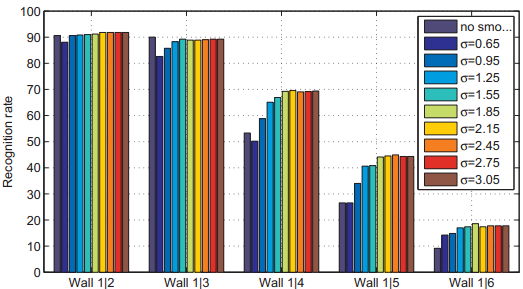
\includegraphics[scale=1]{pict/02/brief/sigma_comp.png}
\caption{Skuteczność rozpoznawania deskryptorów w zależności od stopnia wstępnego rozmycia obrazu}
\label{fig:brief_sigma_comp}
\end{figure}


Twórcy algorytmu zdecydowali się na zastosowanie rozmycia Gaussa. W trakcie prac nad algorytmem badano wpływ promienia rozmycia na jakość deskryptora i jego wydajność. Na zbiorze testowym Mikołajczyka\footnote{Zbiór testowy Mikołajczyka jest szerzej omówiony w rozdziale poświęconym badaniom} przetestowano promienie o zakresie od 0 do 3. Jak pokazuje wykres \ref{fig:brief_sigma_comp} w przedziale promieni od 1 do 3 jakość jest bardzo zbliżona. Finalnie w algorytmie zastosowano dyskretne jądro rozmycia o wartości $\sigma = 2 $ i rozmiarze 9 na 9 pikseli.

\subsection{Wybór testowanych par punktów}
Kluczowe znaczenie dla jakości generowanych deskryptorów, ma dobór par punktów poddawanych testowaniu. Od wyboru metody ich losowania zależy stopień powtarzalności i odporności deskryptora na rotacje. 

W trakcie prac nad algorytmem autorzy przetestowali 5 sposobów selekcji par:
\begin{enumerate}
\item[G I] Lokalizacja punktów \textbf{X} i \textbf{Y} ma rozkład jednostajny na przedziale $(-\frac{S}{2},\frac{S}{2})$. Początek układu współrzędnych umiejscowiony jest w punkcie centralnym badanego obszaru $S\times S$. 
\item[G II] Zbiory punktów \textbf{X} i \textbf{Y} mają rozkład normalny o wartości oczekiwanej 0 i wariancji $\frac{S^2}{25}$. Wartość wariancji została dobrana eksperymentalnie i dla przedstawionej metody zapewnia najwyższy współczynnik rozpoznawalności.
\item[G III] W przypadku tej metody próbkowanie odbywa się 2 etapowo. W pierwszej kolejności z rozkładem normalnym o wartości oczekiwanej 0 i wariancji $\frac{S^2}{25}$ wybierane są punkty \textbf{X}. Punkty \textbf{Y} są lokalizowane w otoczeniu odpowiadających im punktów $x_i$.  \textbf{Y} ma rozkład normalny o wartości oczekiwanej $x_i$ i wariancji $\frac{S^2}{100}$. W przypadku lokalizacja punktu $y_i$ wypada poza badany obszar $S\times S$ przypisuje mu się położenie na krawędzi. Zastosowana metoda powoduje, że badane pary są badane w sposób bardziej lokalny. Podobnie jak w poprzedniej metodzie wartości wariancji zostały dobrane eksperymentalnie.
\item[G IV] Punkty $x_i$ i $y_i$ są wybierane w sposób losowy z dyskretnego zbioru zgrubnych współrzędnych biegunowych.
\item[G V] Wszystkie punkty $x_i$ znajdują się w początku układu współrzędnych a punkty $y_i$ lokalizowane są na liniach zgrubnych współrzędnych biegunowych.
\end{enumerate}

Zaproponowane metody próbkowania zostały przebadane na zbiorze testowym Mikołajczyka. Rezultaty tych badań przedstawione zostały na wykresie \ref{fig:brief_G_comp}. Otrzymane wyniki dowodzą wysokiej skuteczności metod opartych o losowy dobór par. Na ich tle wyjątkowo słabo wypada regularna i symetryczna metoda G V. W ostatecznej wersji algorytmu zdecydowano się zastosować strategie próbkowania G II.
\begin{figure}
\centering

\subfigure[G I]{
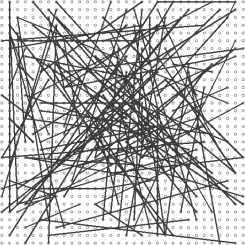
\includegraphics{pict/02/brief/G1.png}
}
\subfigure[G II]{
\includegraphics{pict/02/brief/G2.png}
}
\subfigure[G III]{
\includegraphics{pict/02/brief/G3.png}
}
\subfigure[G IV]{
\includegraphics{pict/02/brief/G4.png}
}
\subfigure[G V]{
\includegraphics{pict/02/brief/G5.png}
}
\caption{Przegląd metod losowania par punktów do testu binarnego}
\label{fig:brief_dist}
\end{figure}

\begin{figure}
\centering
\includegraphics[scale=1]{pict/02/brief/G_comp.png}
\caption{Skuteczność metod losowania par badana na zbiorze Mikołajczka WALL}
\label{fig:brief_G_comp}
\end{figure}

\FloatBarrier
\newpage
\section{Algorytm ORB}
Algorytm ORB jest rozwinięciem wcześniej omówionych algorytmów: FAST i BRIEF. Został on opracowany podobnie jak algorytm STAR w laboratorium robotyki Willow Garrage \cite{ORB11}. 

\subsection{Lokalizowanie punktów charakterystycznych}
Do lokalizowania punktów charakterystycznych algorytm ORB wykorzystuje zmodyfikowany detektor FAST. Jedna z modyfikacji polega na dodaniu do lokalizowanego punktu składowej określającej jego orientacje, dlatego nowy detektor nazwano oFAST (od ang. oriented FAST).


\begin{figure}
\centering
\includegraphics[width=0.8\textwidth]{pict/02/orb/orb_wykres_2.png}
\caption{podpis}
\label{fig:orb_wykres_2}
\end{figure}

\begin{figure}
\centering
\includegraphics[width=0.8\textwidth]{pict/02/orb/orb_wykres_3.png}
\caption{podpis}
\label{fig:orb_wykres_3}
\end{figure}


\begin{figure}
\centering
\includegraphics[width=0.8\textwidth]{pict/02/orb/orb_wykres_4.png}
\caption{podpis}
\label{fig:orb_wykres_4}
\end{figure}


\begin{figure}
\centering
\includegraphics[width=0.8\textwidth]{pict/02/orb/orb_wykres_5.png}
\caption{podpis}
\label{fig:orb_wykres_5}
\end{figure}



\begin{figure}
\centering
\includegraphics[width=0.8\textwidth]{pict/02/orb/orb_wykres_6.png}
\caption{podpis}
\label{fig:orb_wykres_6}
\end{figure}


\begin{figure}
\centering
\includegraphics[width=0.8\textwidth]{pict/02/orb/orb_wykres_7.png}
\caption{podpis}
\label{fig:orb_wykres_7}
\end{figure}


\begin{figure}
\centering
\includegraphics[width=0.8\textwidth]{pict/02/orb/orb_wykres_8.png}
\caption{podpis}
\label{fig:orb_wykres_8}
\end{figure}

Pierwszym krokiem w działaniu algorytmu jest "zgrubne" zlokalizowanie punktów charakterystycznych. Realizuje się to za pomocą detektora FAST-9, gdzie 9 oznacza ilość ciągłych pikseli w okręgu lokalizującym róg.

Oryginalny algorytm FAST nie dostarcza żadnej miary jakości zlokalizowanego rogu,  skutkiem czego jest dosyć wrażliwy na zakłócenia spowodowane odpowiedzią krawędziową. W efekcie bardzo często dostajemy bardzo dużą liczbę punktów charakterystycznych, niestety o słabej jakości. 

Rozwiązaniem powyższego problemu jest zastosowanie detektora Harrisa do oceniania punktów charakterystycznych. Algorytm ORB jako jeden z argumentów przyjmuje pożądaną liczbę punktów charakterystycznych oznaczoną przez N. Znając liczbę N algorytm tak ustala się wartość progu miary Harrisa aby uzyskać zbiór punktów, których ilość przekracza N. Następnie zbiór ten jest sortowany i wybiera się z niego N najlepszych punktów. W zastosowaniach praktycznych wartość liczby N ustala się najczęściej na 500. Zwiększenie tej liczby powoduje otrzymanie większej liczby punktów charakterystycznych, ale często gorszej jakości i nachodzące na punkty z grupy pięciuset.

Kolejnym wadę algorytmu FAST jest jego wrażliwość na skalowanie obrazu. W przypadku detektora oFAST zastosowano omawiany wcześniej mechanizm piramidy skalo-przestrzennej.

Do określenia orientacji rogu będącego punktem charakterystycznym zastosowano miarę intensywności środka ciężkości \cite{centroid}. Metoda ta zakłada, że intensywność rogu jest przesunięta względem jego środka. Wektor przesunięcia jest używany do określenie orientacji punktu charakterystycznego. 

Definiując dla badanego wycinka momenty jako:
\begin{equation}
m_{pq} = \sum\limits_{x,y} x^p y^q I(x,y)
\end{equation}
i środek ciężkości:
\begin{equation}
C = \left(\frac{m_{10}}{m_{00}},\frac{m_{01}}{m_{00}}\right)
\end{equation}
możemy skonstruować wektor $\overrightarrow{OC}$ zaczepiony w środku rogu i skierowany w stronę środka ciężkości. Orientacje tego wektora możemy w prosty sposób obliczyć z zależności:
\begin{equation}
\theta = atan2(m_{01},m_{10})
\end{equation}

Aby poprawić stabilność zaprezentowanej miary na rotacje, punkty $x$ i $y$ są wybierane z kołowego obszaru o promieniu $r$. W praktyce oznacza to, że $r$ reprezentuje rozmiar badanego wycinka a współrzędne $x$ i $y$ zawierają się w przedziale [-r,r]. W sytuacji gdy wartość momentu badanego odcinka |C| wynosi 0 algorytm zachowuje się w sposób niestabilny. W przypadku punktów lokalizowanych przez algorytm FAST jest to jednak bardzo rzadki przypadek.

Zaprezentowana metoda została porównana z metodami bazującymi na gradiencie obrazu, BIN i MAX. Metoda MAX wybiera największa składową gradientu w obrębie badanego punktu. Metoda BIN podobnie jak w algorytmie SIFT i jest oparta o histogram reprezentujący wszystkie składowe gradientu. Jak pokazuje wykres \ref{fig:orb_wykres_2} metoda oparta o środek ciężkości jest o znacznie bardziej odporna na zakłócenia.
\subsection{Budowa deskryptora}
Do opisu zlokalizowanych cech wykorzystano ulepszoną zmodyfikowaną wersje deskryptora Steered BRIEF nazwaną rBRIEF. 

Steered Brief jest rozwinięciem opisanego wcześniej deskryptora BRIEF. Oryginalny deskryptor BRIEF jest bardzo wrażliwy na rotacje [wykres \ref{fig:orb_wykres_7}]. Pewnym rozwiązaniem, aczkolwiek bardzo nieoptymalnym, jest zaproponowane przez autorów algorytmu BRIEF wyliczenie grupy obróconych względem siebie deskryptorów. Znacznie lepszym rozwiązaniem dostrojenie deskryptora BRIEF do orientacji punktu charakterystycznego. Deskryptor BRIEF jest generowany przez $n$ testów binarny dla zbioru par punktów ($x_i$,$y_i$). Zbiór ten jest opisany przez macierz $\textbf{S}$:
\begin{equation}
\textbf{S} = \left(\begin{array}{ccccccc}
x_1 & , & x_2 & , & ... & , & x_n \\
y_1 & , & y_2 & , & ... & , & y_n \\
\end{array}
\right)
\end{equation} 

Na podstawie obliczonej wcześniej orientacji punktu charakterystycznego $\theta$ i odpowiadającej jej macierzy rotacji $\textbf{R}_{\theta}$, konstruowany jest "ukierunkowany" zbiór testowy $\textbf{S}_{\theta}$:

\begin{equation}
\textbf{S}_\theta = \textbf{R}_\theta \textbf{S}
\end{equation}

Otrzymany zbiór jest poddawany temu samemu testowi jak w przypadku oryginalnego algorytmu BRIEF (wzór \ref{eqn:brief_test}).

W celu usprawnienia pracy algorytmu orientacje punktów charakterystycznych poddawane są kwantyzacji. Dla zakresu $360^o$ przyjęto się 30 przedziałów $12^o$ do których może zostać zakwalifikowana orientacja punktu. Każdy z przedziałów posiada własny wzorzec punktów poddawanych testom.

Jedną z niewątpliwych zalet algorytmu BRIEF jest to że każdy bit jego deskryptora ma dużą wariancje i wartość średnią na poziomie $0,5$. Wykres \ref{fig:orb_wykres_3} prezentuje rozrzut wartości średniej dla typowego gaussowskiego wzorca 256 bitowego deskryptora BRIEF dla zbioru 100 tysięcy punktów charakterystycznych. Wartość średnia $0,5$ daje największą wariancje próbkowania na poziomie $0,25$ dla pojedynczego bitu. Zastosowanie "ukierunkowanego" algorytmu BRIEF powoduje przesunięcie wartości średniej w stronę rozkładu typowego dla wzorca odpowiadającego danemu kątowi orientacji. Powoduje to zbytnie upodobnienie się deskryptorów punktów zakwalifikowanych do tego samego przedziału orientacji.

Wysoka wariancje czyni deskryptory bardziej dyskryminacyjnymi co jest pożądanym zjawiskiem, gdyż generuje bardziej zróżnicowane odpowiedzi dla punktów o podobnych parametrach. 

Kolejnym ważnym aspektem  jest również to aby kolejne bity deskryptora były ze sobą nieskorelowane. Autorzy algorytmu dla badanego zbioru 100 tysięcy punktów dokonali analizy głównych składowych (ang. PCA) otrzymywanych deskryptorów. Wyniki tego badania przedstawia wykres \ref{fig:orb_wykres_4}. Na podstawie analizy wykreślono 40 najwyższych wartości własnych, po których zarówno deskryptory BRIEF jak steered BRIEF się pokrywają. Obie motody wykazują wysokie wejściowe wartości własne, wskazujące na korelacje testów binarnych. Większość informacji jest zawarta w pierwszych 15 komponentach. Algorytm steered BRIEF ma znacznie mniejszą wariancję, aczkolwiek przy mniejszych wartościach własnych przestaje być dyskryminacyjnym. Na podstawie tego można stwierdzić, że BRIEF zawdzięcza swoja dobre wyniki losowej orientacji punktów charakterystycznych.

Innym niekorzystnym efektem towarzyszącym deskryptorowi steered BRIEF jest zmniejszenie dystansu miedzy punktami pokrywającymi się i odstającymi co przedstawiono na wykresie \ref{fig:orb_wykres_5}. Może to powodować nie pożądane nachodzenie na siebie punktów poprawnych i złych, a co za tym idzie powodować fałszywe dopasowania.

Aby zapobiec opisanym zjawiskom spadku wariancji i wzrostu korelacji pomiędzy testami, autorzy algorytmu zaproponowali metodę uczenia służącą wyborowi dobrego podzbioru binarnych testów.

W zaproponowanej metodzie na podstawie zbioru obrazów PASCAL 2006 \cite{pascal} przygotowano zbiór uczący zawierający około 300 tysięcy punktów charakterystycznych. Następnie dla okna o wymiarach $31\times31$ pikseli przygotowano kombinacje wszystkich możliwych binarnych testów. Każdy test jest jest wykonywany na parze mniejszych okien $5\times5$. Zapisując szerokość dużego okna jako $w_p = 31$ i szerokość małego okna jako $w_t = 5$ otrzymujemy liczbę $N = (w_p - w_t)^2$ oznaczającą liczbę możliwych małych okien. Wybierając 2 okna do pojedynczego badania otrzymujemy zbiór ${N\choose 2}$ testów. Eliminując testy nakładające się na siebie otrzymujemy zbiór 205590 porównań.

Przygotowany zbiór uczący poddano badaniu następującemu algorytmowi:
\begin{enumerate}
\item Wszystkie obrazy zbioru uczącego przetestowano wszystkimi kombinacjami testów.
\item Testy zostały uporządkowane na podstawie odległości wartości średniej od wartości $0,5$ i zawarte w wektorze \textbf{T}.
\item Następnie wektor \textbf{T} jest poddawany przeszukiwaniu zachłannemu:
\begin{enumerate}
\item Pierwszy test wektora \textbf{T} jest kopiowany do 256 wymiarowego wektora \textbf{R} i usuwany ze zbioru \textbf{T}.
\item Kolejny test ze zbioru \textbf{T} jest porównywany ze wszystkimi testami znajdującymi w wektorze \textbf{R}. W sytuacji gdy wartość absolutna korelacji między testami jest mniejsza niż zadany próg, test zostaje przeniesiony do zbioru wektora \textbf{R}.
\item Punkt (b) jest powtarzany aż do momenty, w którym w wektor \textbf{R} będzie posiadał 256 elementów. W sytuacji niespełnienia warunku stopu i wyczerpania się elementów wektora \textbf{T} wartość progu jest podnoszona i algorytm powtarza swoje działanie.
\end{enumerate}
\end{enumerate}
Wynik działania tego algorytmu został nazwany rBRIEF. Algorytm ten ma znacząco lepsze parametry wariancji i korelacji niż algorytm steered BRIEF. Jak przedstawia wykres \ref{fig:orb_wykres_4} wygenerowany deskryptor ma wartości własne głównych składowych są wyższe i zmniejszają się znacznie wolniej niż w przypadku algorytmów steered BRIEF i BRIEF. Badania przeprowadzone przez autorów algorytmów wykazują ponadto wysoką odporność na rotacje [wykres \ref{fig:orb_wykres_7}].